\chapter{Umsetzung}

\section{Motoransteuerung}
Wie bereits im Konzept beschrieben, wird der Motorteiber als diskreter Vierquadrantensteller ausgeführt. Auf Grund der hohen Belastbarkeit
und leistungslosen Ansteuerung werden meist p-Kanal-Mosfets als Halbleiterschalter genutzt. Um die beiden oberen Mosfets (T1/T3) durchzuschalten
ist auf Grund des fehlenden Massepotentials eine Gatespannung oberhalb der Betriebsspannung nötig. Diese wird meist mittels Bootstrapping zur
Verfügung gestellt. Da das simultane Durchschalten der übereinander liegenden Mosfets zu einem Kurzschluss führen würde, muss dies durch
eine Schutzschaltung verhindert werden. Um all diese Funktionen zur Verfügung zu stellen gibt es bereits fertige Mosfettreiber,
welche das Schaltungsdesign enorm vereinfachen.

\begin{figure}[H]
\centering
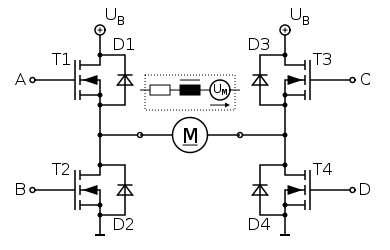
\includegraphics[width=.8\textwidth]{Vierquadrantensteller.png}\\
\caption{Vierquadrantensteller \cite{vierquadrantensteller}}%
\label{fig:Vierquadrantensteller}
\end{figure}

\subsection{Auswahl der Mosfets}
Die Auswahl der Mosfets wird durch den geforderten Strom von \SI{20}{\ampere} und der maximalen Betriebsspannung von \SI{20}{\volt} eingegrenzt. Weitere Kriterien wie die Gate-Source-Spannung, welche zum Durchschalten
der Mosfets benötigt wird, sind auf Grund der Tatsache, dass ein Mosfettreiber verwendet werden soll nicht von Belang, da dieser die benötigten Spannungen generiert.
Für die Anwendung in einem Vierquadrantensteller ist die wahrscheinlich wichtigste Größe der Drain-Source-Widerstand im Einschaltzustand $R_{\text{DS(ON)}}$.
Ein kleiner $R_{\text{DS(ON)}}$ ist von Vorteil und führt zu einer kleinen Verlustleistung an den Mosfets.
Mosfets mit einem hervorragenden $R_{\text{DS(ON)}}$ von nur \SI{12}{\milli\ohm} sind die FDD6690A von Fairchild Semiconductor \cite{ds-fs}. Weitere Kenngrößen dieser sind
eine maximale Drain-Source-Spannung von \SI{30}{\volt} sowie eine Belastbarkeit von \SI{46}{\ampere}, eine gute Kühlung vorausgesetzt. Aufgrund der kleinen Gate Ladung von \SI{13}{\nano\coulomb} eignen
sie sich gut für hohe Schaltfrequenzen. Aufgrund ihres niedrigen $R_{\text{DS(ON)}}$ werden sie für die Platine genutzt.


\subsection{Mosfettreiber}

\subsubsection{Verfügbarkeit}

Mosfettreiber gibt es in vielen Ausführungen, unter anderem als ``Single Channel High Side Driver``, ``Half Bridge Driver'', ``Full Bridge Driver''
und ``3 Phase Driver''. Da für den verbauten DC-Motor eine Vollbrücke nötig ist, um den Motor in alle Richtungen zu betreiben, werden an dieser Stelle
ausschließlich ``Full Bridge Driver'' untersucht.

Eine Tabelle auf Mikrocontroller.net\cite{FET_D_TABLE} zeigt eine Auswahl an ver\-füg\-ba\-ren Mosfettreibern. Dort sind zwei
``Full Bridge Driver'' aufgeführt, welche für dieses Projekt passend sind. Allerdings fällt die Entscheidung auf einen anderen Treiber,
dem Allegro A3941 \cite{ds-A3941}.
\subsubsection{Allegro A3941}
Der Allegro A3941  ist für Betriebsspannungen von \SI{5,5}{\volt} bis \SI{50}{\volt} geeignet und liegt damit in der Spezifikation des Projekts.
Des Weiteren verfügt der Motor über einen integrierten \SI{5}{\volt}-Regulator und kann somit ohne Spannungsregulator am Akku betrieben werden.
Über zwei Ausgänge der Treibers können diverse Fehler ausgelesen werden. Auch sind alle gängigen Schutzschaltungen wie z.B. ein Kurzschlussschutz enthalten.
Daher ist er hervorragend für das Projekt geeignet.


Der Treiber lässt sich in verschiedenen Modi betreiben:

\begin{figure}[H]
\centering
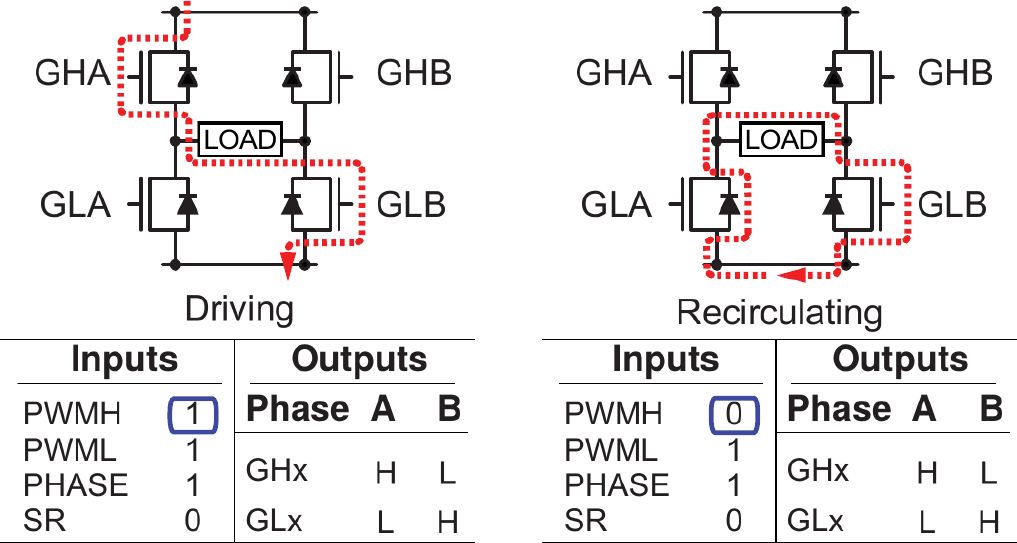
\includegraphics[width=.8\textwidth]{3941_1.png}\\
\caption{Slow decay, diode recirculation, high-side PWM \cite{ds-A3941}}%
\label{fig:39411}
\end{figure}

Konfiguration: PWML=1, PHASE=1, SR=0 und PWM an PWMH (high-side PWM)\\
Bei aktivierten PWMH fließt der Strom durch den GHA-Mosfets über den Motor und
dann über den GLB-Mosfet. In diesem Modus wird der Motor angetrieben.
Wenn PWML deaktiviert ist, zirkuliert der vom Motor induziert Strom durch GLB und durch
die interne Diode von GLA, der Motor wird dadurch gebremst.


\begin{figure}[H]
\centering
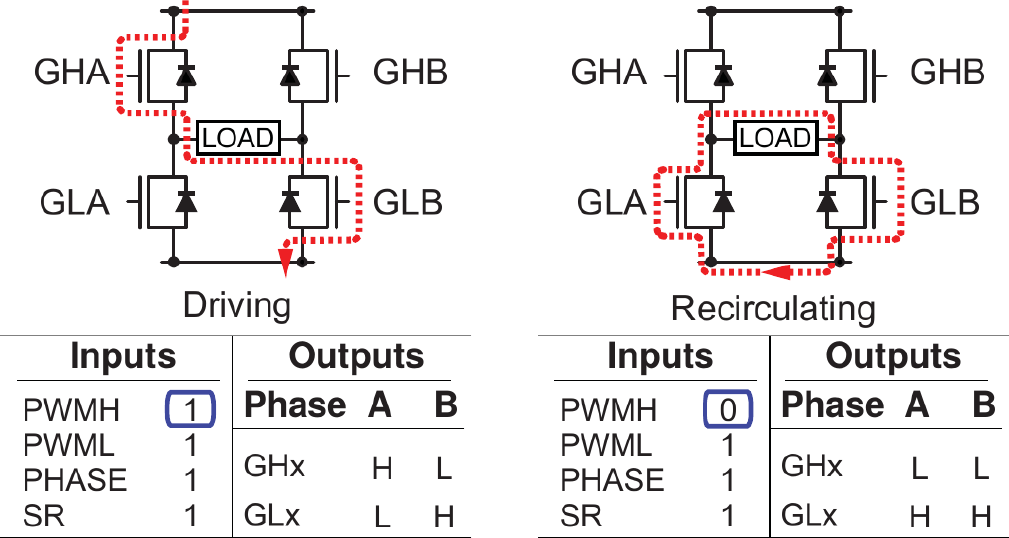
\includegraphics[width=.8\textwidth]{3941_2.png}\\
\caption{Slow decay, SR active, high-side PWM \cite{ds-A3941}}%
\label{fig:39412}
\end{figure}

Konfiguration: PWML=1, PHASE=1, SR=1 und PWM an PWMH (high-side PWM)\\
Bei aktivierten PWMH fließt der Strom durch den GHA-Mosfets über den Motor und
dann über den GLB-Mosfet. In diesem Modus wird der Motor angetrieben.
Wenn PWML deaktiviert ist, zirkuliert der vom Motor induziert Strom durch 
GLB und durch GLA. Der Motor wird durch den niedrigeren Innenwiderstand des Mosfets 
stärker gebremst als in der vorherigen Konfiguration. Dabei ist darauf zu achten, dass
beinahe die gesamte vom Motor induzierte Spannung über den beiden Mosfets (GLA/GLB) abfällt,
was zu einer starken Hitzeentwicklung führen kann.



\begin{figure}[H]
\centering
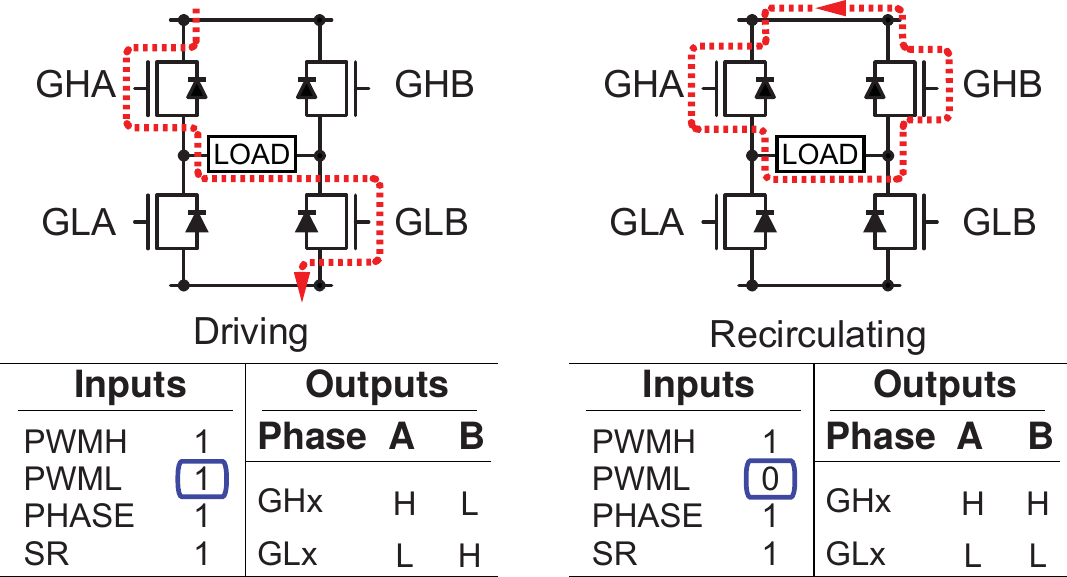
\includegraphics[width=.8\textwidth]{3941_3.png}\\
\caption{Slow decay, SR active, low-side PWM \cite{ds-A3941}}%
\label{fig:39413}
\end{figure}

Konfiguration: PWMH=1, PHASE=1, SR=1 und PWM an PWML (low-side PWM)\\
Diese Konfiguration entspricht im Grunde den beiden vorherigen, nur dass das PWM-Signal
an den unteren Mosfets anliegt. Der SR-Pin entscheidet wieder darüber ob im ``Bremsmodus''
die internen Dioden genutzt werden (SR=0) oder nicht (SR=1).




\begin{figure}[H]
\centering
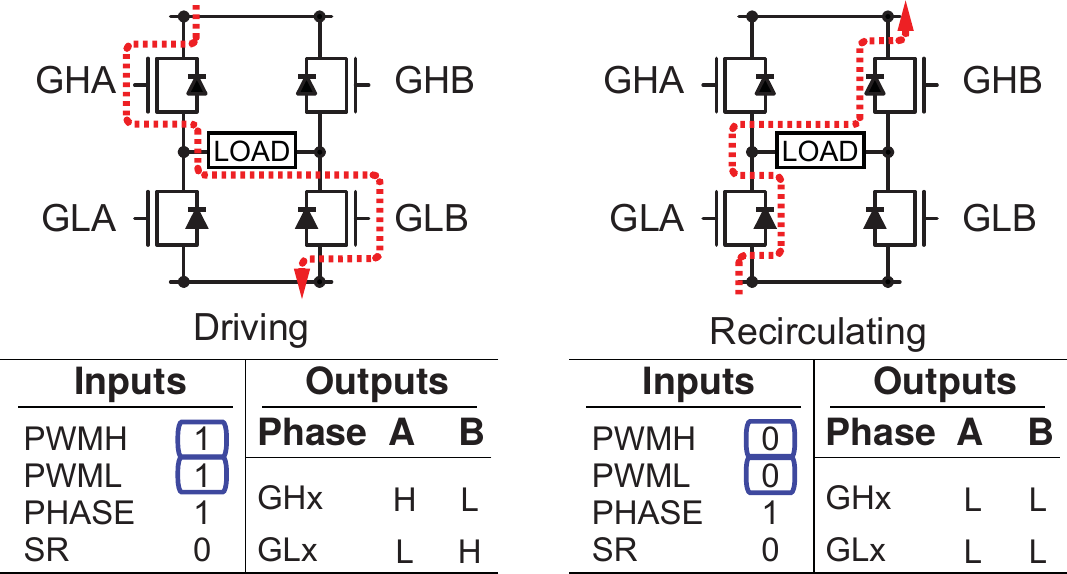
\includegraphics[width=.8\textwidth]{3941_4.png}\\
\caption{Fast decay, diode recirculation \cite{ds-A3941}}%
\label{fig:39414}
\end{figure}


Konfiguration: PWMH=1, PWML=1, PHASE=1, SR=1\\
In dieser Konfiguration werden die oberen und unteren Mosfets gleich geschaltet. Im
``Bremsmodus'' führt das dazu, dass der induzierte Motorstrom nicht über die Mosfets
zirkulieren kann. Der Strom fließt stattdessen zurück in die Spannungsquelle, was
abhängig von der Spannungsquelle zu Schäden führen kann. Wird die Schaltung jedoch an
einem geeigneten Akku betrieben, ist es so möglich die Energie zu nutzen und damit den Akku
zu laden.

\begin{figure}[H]
\centering
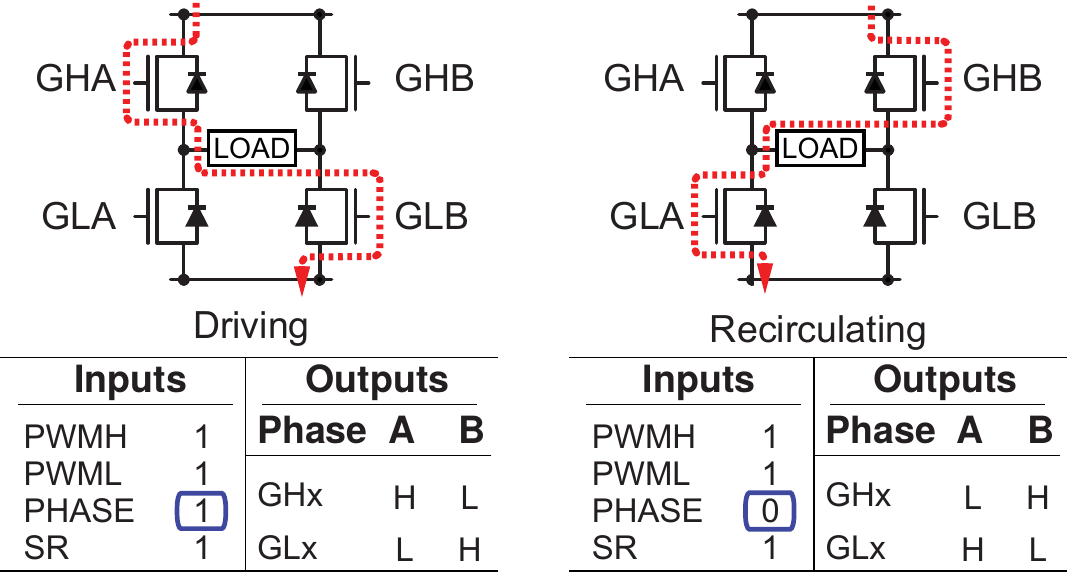
\includegraphics[width=.8\textwidth]{3941_5.png}\\
\caption{Fast decay, SR active, full four-quadrant control \cite{ds-A3941}}%
\label{fig:39415}
\end{figure}

Diese Konfiguration zeigt den Einfluss des PHA\-SE-Pins. Liegt am PHA\-SE-Pin 1 an,
fließt der Strom von links nach rechts. Liegt 0 an, fließt er von rechts nach links.
Mithilfe des PHASE-Pins wird also die Polung des Motors festgelegt.


\subsubsection{Schaltplan}

In Folgenden wird geklärt wie sich die Beschaltung des Allegro A3941 bestimmen lässt. Die Schaltung in \cref{fig:schalt:allegro} entspricht dabei den Vorgaben im Datenblatt.

\begin{figure}[H]
\centering
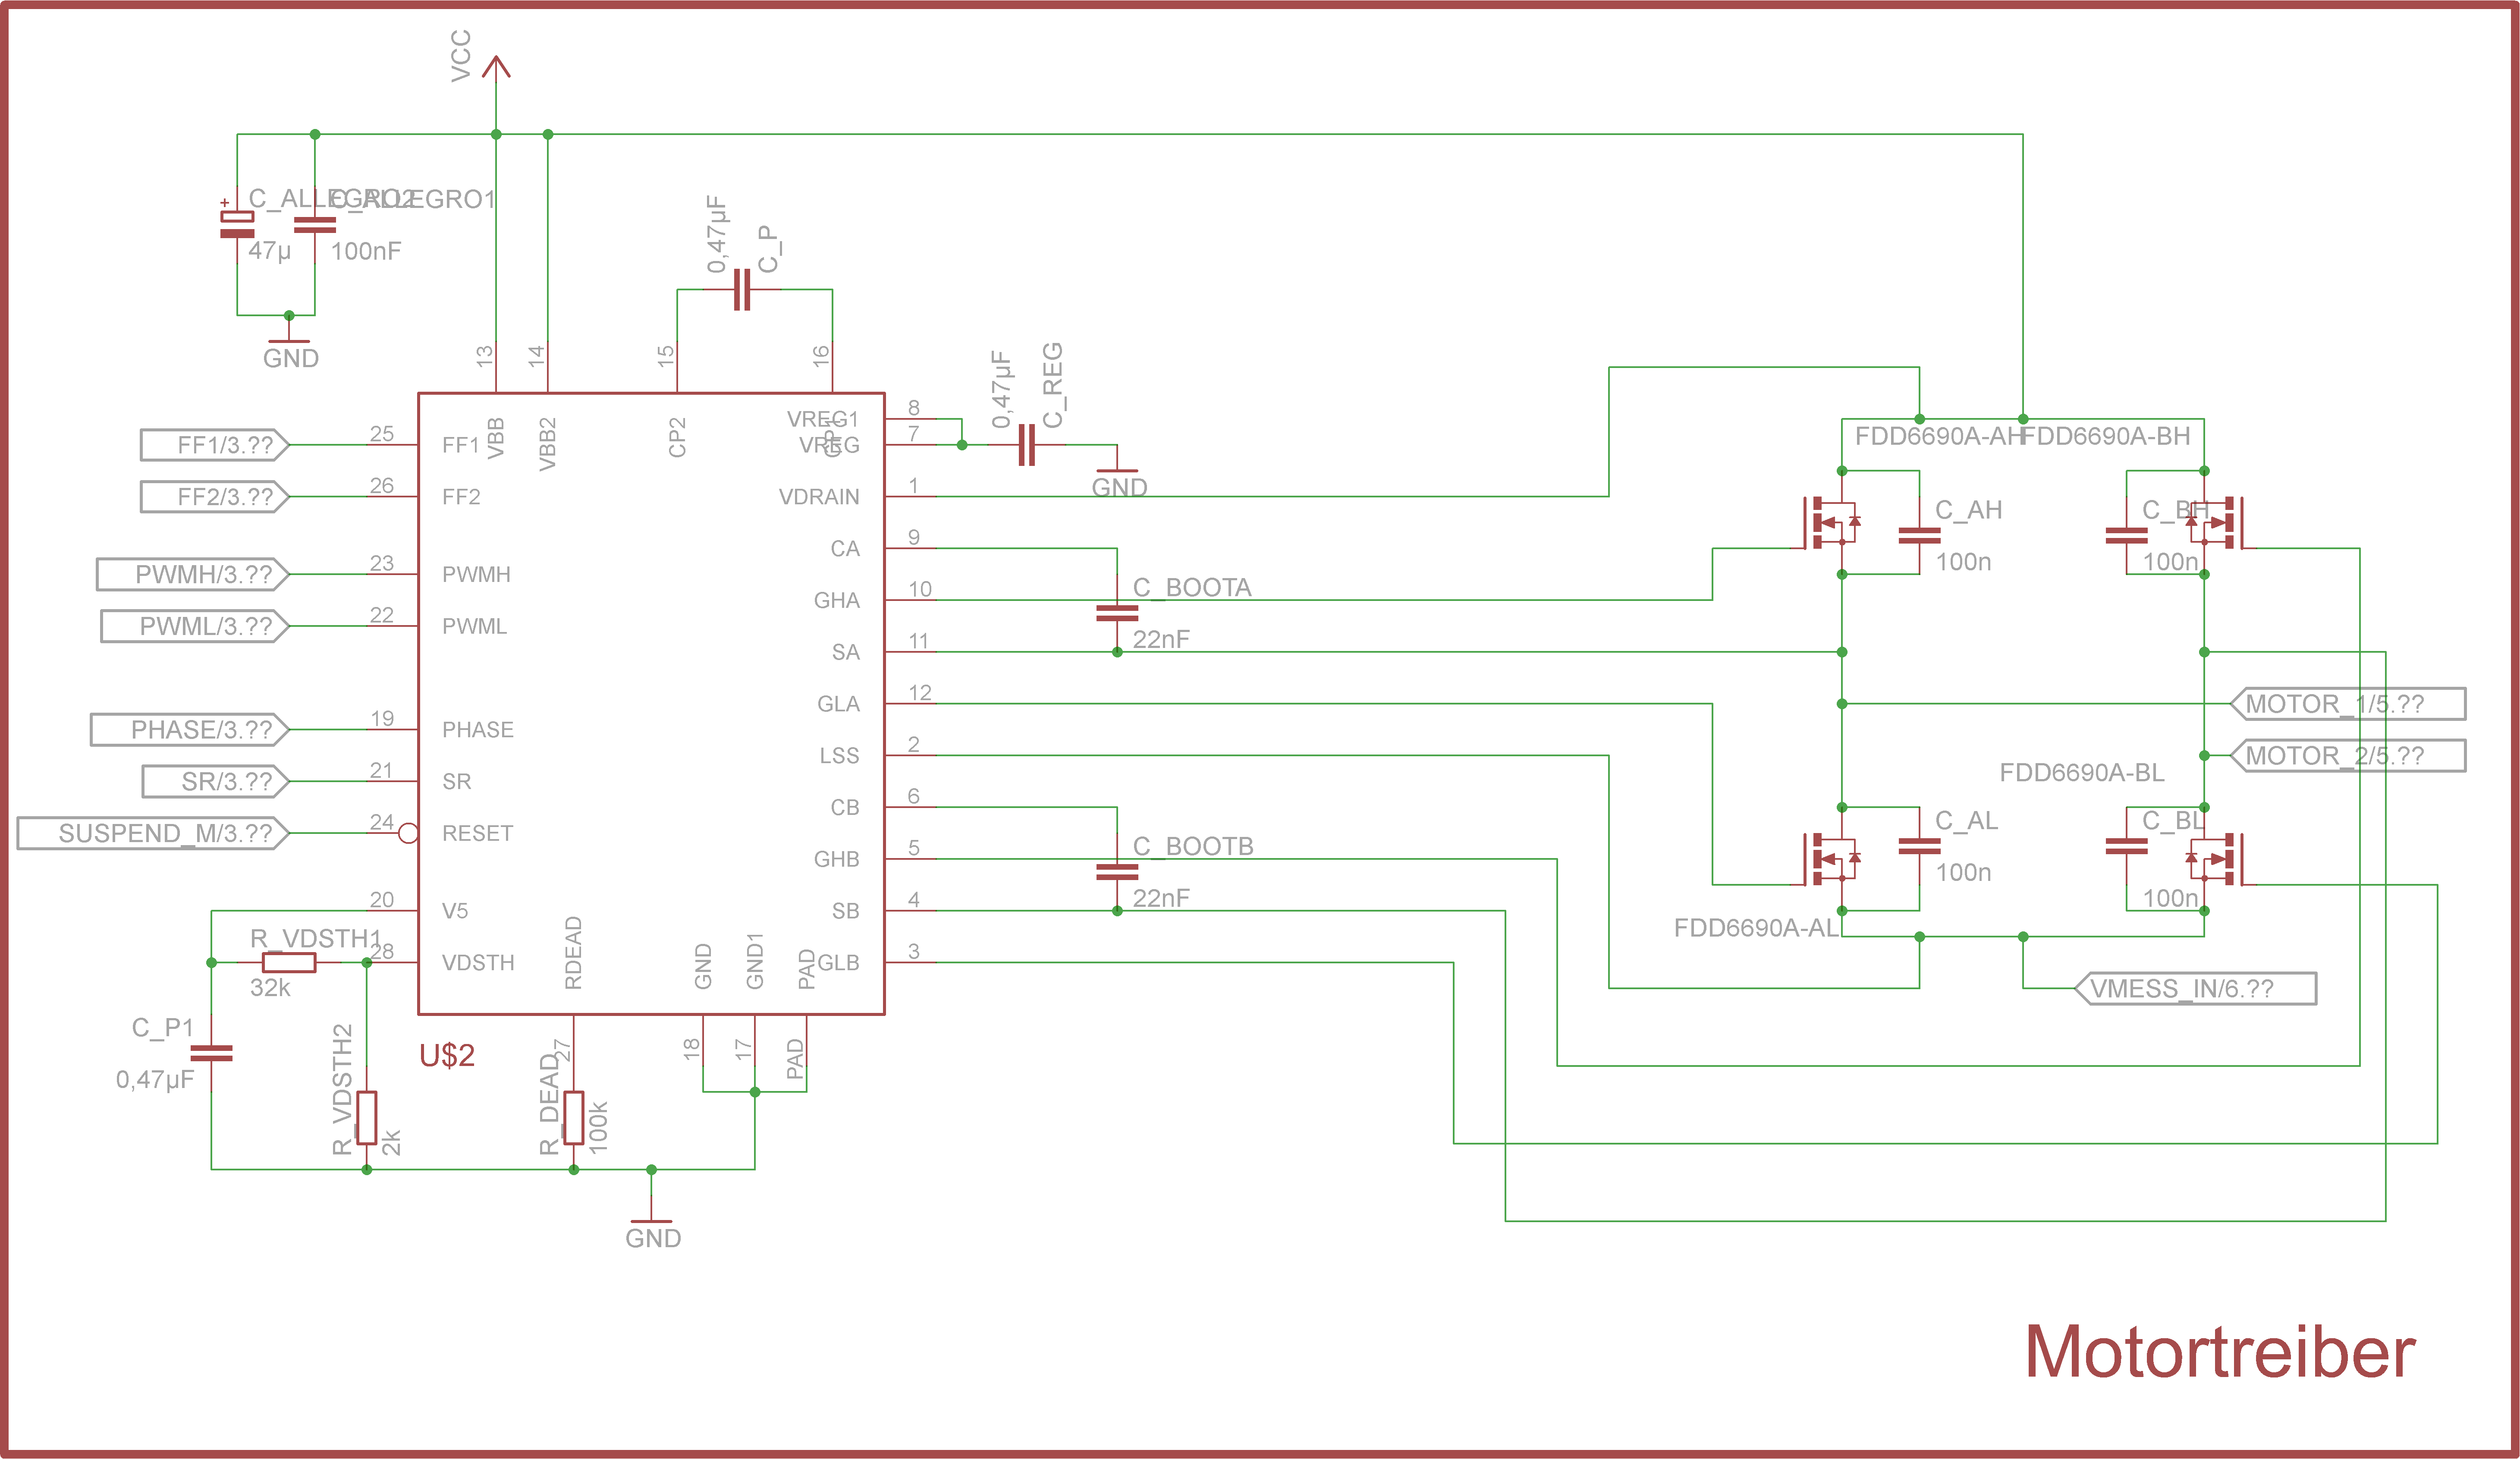
\includegraphics[width=\textwidth]{motortreiber.png}\\
\caption{Schaltplan Allegro A3941}%
\label{fig:schalt:allegro}
\end{figure}

$R_{\text{DEAD}}$ legt die Totzeit zwischen den Mosfetumschaltungen fest. Wird sie zu niedrig gewählt, können in jeder PWM-Periode Kurzschlüsse auftreten. Wird sie zu hoch
gewählt, beschränkt man das Tastverhältnis unnötig, was die Motorleistung reduziert. Da wir ``Low Gate Charge'' Mosfets nutzen und die Einschalt- bzw. Ausschaltzeit
der Mosfets hauptsächlich von dieser Größe abhängt, ist diese Zeit sehr klein. Eine genaue Bestimmung dieser Zeit ist sehr aufwändig, deswegen
wird hier ein mittlerer Wert von \SI{100}{\kilo\ohm} gewählt, dieser soll sich laut Datenblatt zwischen 3 und \SI{240}{\kilo\ohm} befinden.\\


%(ca 50ns).
%
% 
% Die Totzeit t\textsubscript{DEAT} bestimmt sich folgender Maßen (für 3-240k$\Omega$)
% 
% \begin{align*}
% t_{\text{DEAD}}=50+\frac{7200}{1.2+200/R_{\text{DEAD}}} %100k
% \end{align*}
% 
% Ein Widerstand von 3k$\Omega$ resultiert in einer Totzeit von 106ns was einen guten Wert darstellt.


% $R_{\text{DEAD}}$ legt die Totzeit zwischen den Mosfetumschalungen fest. Wird es zu niedrig gewählt können in jeder PWM-Periode Kurzschlüsse auftreten. Wird es zu hoch
% gewählt beschrängt man das Tastverhältnis unnötig, was die Motorleistung reduziert. Um die Ideale Totzeit festzulegen muss die lade bzw entlade Dauer der 
% Mosfetgates bestimmt werden. Die Gateladung der Mosfets beträgt 13nC bei 5V. Da die Mosffets über $V_{REG}$ geladen werden beträgt die
% Gatekapazität $C_{\text{GATE}}=\frac{13nC}{13V}=1\text{nF}$. Die Entladedauer für für einen nF beträgt laut Datenblatt 20ns. Die Ladedauer 35ns. Allerdings ist

Als Nächstes werden die Größen der Bootstrapkondensatoren C\textsubscript{BOOTA} und C\textsubscript{BOOTB} bestimmt. Diese sind für eine ordnungsgemäße
Funktion der Schaltung richtig zu wählen. Zu kleine Kondensatoren verhindern ein Durchschalten der oberen Mosfets, was zu einer nicht funktionsfähigen Schaltung
führt. Zu große Werte hingegen verringern das maximale Tastverhältnis des PWM Signals, da die Aufladung der Kondensatoren Zeit in Anspruch nimmt.
Laut Datenblatt hat sich folgende Faustformel gut bewährt:

\begin{align*}
C_{\text{BOOT}}=\frac{Q_{\text{GATE}}\cdot20}{V_{\text{BOOT}}}
\end{align*}


V\textsubscript{BOOT} entspricht dabei in etwa V\textsubscript{REG}, welche laut Datenblatt \cite{ds-A3941} 13V beträgt.
Die Gateladung Q\textsubscript{GATE} der FDD6690A Mosfets beträgt typischerweise \SI{13}{\nano\coulomb} \cite{ds-fs}. Damit ergibt sich für C\textsubscript{BOOT}=20nF. Es werden demnach
die nächst größeren \SI{22}{\nano\farad} als Bootstrapkondensatoren genutzt.\\

Die Spannung V\textsubscript{DSTH} am VDSTH-Eingang soll der Spannung entsprechen die maximal über jeden Mosfet abfallen darf, bevor der Treiber einen Kurzschuss detektiert 
und abschaltet. Da der maximale Strom durch unseren Motor \SI{20}{\ampere} beträgt, lässt sich diese Spannung, einfach berechnen. Der Widerstand der Mosfest im Einschaltzustand beträgt
in unseren Fall ($U_{GS}=\SI{13}{\V}$) etwas weniger als \SI{12}{\milli\ohm}  bei einem Strom von \SI{20}{\A} ergibt sich damit eine Spannung von $\SI{12}{\milli\ohm} \cdot \SI{20}{\A} = \SI{0,24}{\V}$
Da wir den Motor über sein gesamtes Leistungsspektrum nutzen wollen, muss diese Spannung etwas darüber gewählt werden.

Da der Strom in VDSTH nur minimal ist (ca \SI{10}{\micro\ampere}), kann diese Spannung über einen einfachen Spannungsteiler zur Verfügung gestellt werden. Ein Spannungsteiler mit 
Widerständen zu \SI{2}{\kilo\ohm} und \SI{32}{\kilo\ohm} erzeugt uns zusammen mit den \SI{5}{\volt} aus dem V5 Ausgang eine Spannung von $\frac{\SI{2}{\kilo\ohm}}{\SI{32}{\kilo\ohm}+\SI{2}{\kilo\ohm}}\cdot \SI{5}{\V} =\SI{0,24}{\V}$.
Der Spannungsteiler wird durch R\textsubscript{VDSTH1} und R\textsubscript{VDSTH2} gebildet.\\

Die Größe des C\textsubscript{REG} Kondensators hängt direkt mit der Größe der Bootstrapkondensatoren zusammen. Er soll ca 20 mal größer als
C\textsubscript{BOOTA} bzw C\textsubscript{BOOTB} gewählt werden, so dass hier ein \SI{470}{\nano\farad} Kondensator gewählt wird.\\

Das Datenbatt empfiehlt \SI{100}{\nano\farad} entkoppelungs Kondensatoren zwischen Drain und Source eines jeden Mosfets. Diese wurden in Form von C\textsubscript{AH},C\textsubscript{AL},C\textsubscript{BH} und C\textsubscript{BL} 
verbaut. Alle restlichen Größen werden direkt dem Datenblatt entnommen.\\

Da der verwendete AVR Mikrocontroller nur über begrenzte PWM fähige Anschlüsse verfügt, wird lediglich der PWM-Kanal für die oberen Mosfets (PWMH) an einen PWM Ausgang des AVR angeschlossen.
Durch diese Entscheidung werden Betriebsmodi, welche ein Gleichschalten der Mosfets erfordern, erschwert und können nur durch ein Software PWM realisiert werden. Der Vorteil es Betriebsmodus ``Fast decay, diode recirculation''
ist, dass es möglich ist Bremsenergie des Fahrzeugs zurück in den Akku zu speisen. Da die Akkus jedoch mit einer integrierten Ladeelektronik ausgestattet sind, liegt die Vermutung nahe, dass ein Laden des Akkus so nicht möglich ist.
Deshalb wird der Betriebsmodus im Rahmen dieser Arbeit nicht untersucht.

Alle weiteren Anschlüsse des Allegros werden direkt an Pins von PORTC am Mikrocontroller angeschlossen. Da die Fehlerausgänge als Open-Col\-lec\-tor ausgeführt sind, werden die internen Pullup-Widerstände des Mikrocontrollers genutzt.

\section{Motorstrommessung am Shunt}

Da innerhalb des Wettbewerbes Energieeffizienz wichtig ist, ist es notwendig den aktuellen Stromverbrauch zu kennen. Es wird davon ausgegangen, dass der Stromverbrauch der Recheneinheit und Sensoren
konstant ist, bzw.. sich mit der fertigen Software über die Zeit nicht wesentlich ändert. Da der Motor einen großen zu erwartenden Verbrauch hat, ist es wichtig seinen Verbrauch zu bestimmen. Mithilfe dieser
Informationen ist es möglich verschiedene Fahrregler Auslegungen im Aspekt des Verbrauches zu vergleichen. Um den Verbrauch zu bestimmen, ist es notwendig die anliegende Spannung und den Strom durch den
Motor zu messen. Die H-Brücke wird dabei als Teil des Motors betrachtet, daher entspricht Spannung über den Motor der Akkuspannung. Diese lässt sich einfach über einen Spannungsteiler an den ADC des Mikrocontrollers
anschließen. Als Werte für den Spannungsteiler werden \SI{1,8}{\kilo\ohm} und \SI{10}{\kilo\ohm} gewählt.

\begin{figure}[H]
\centering
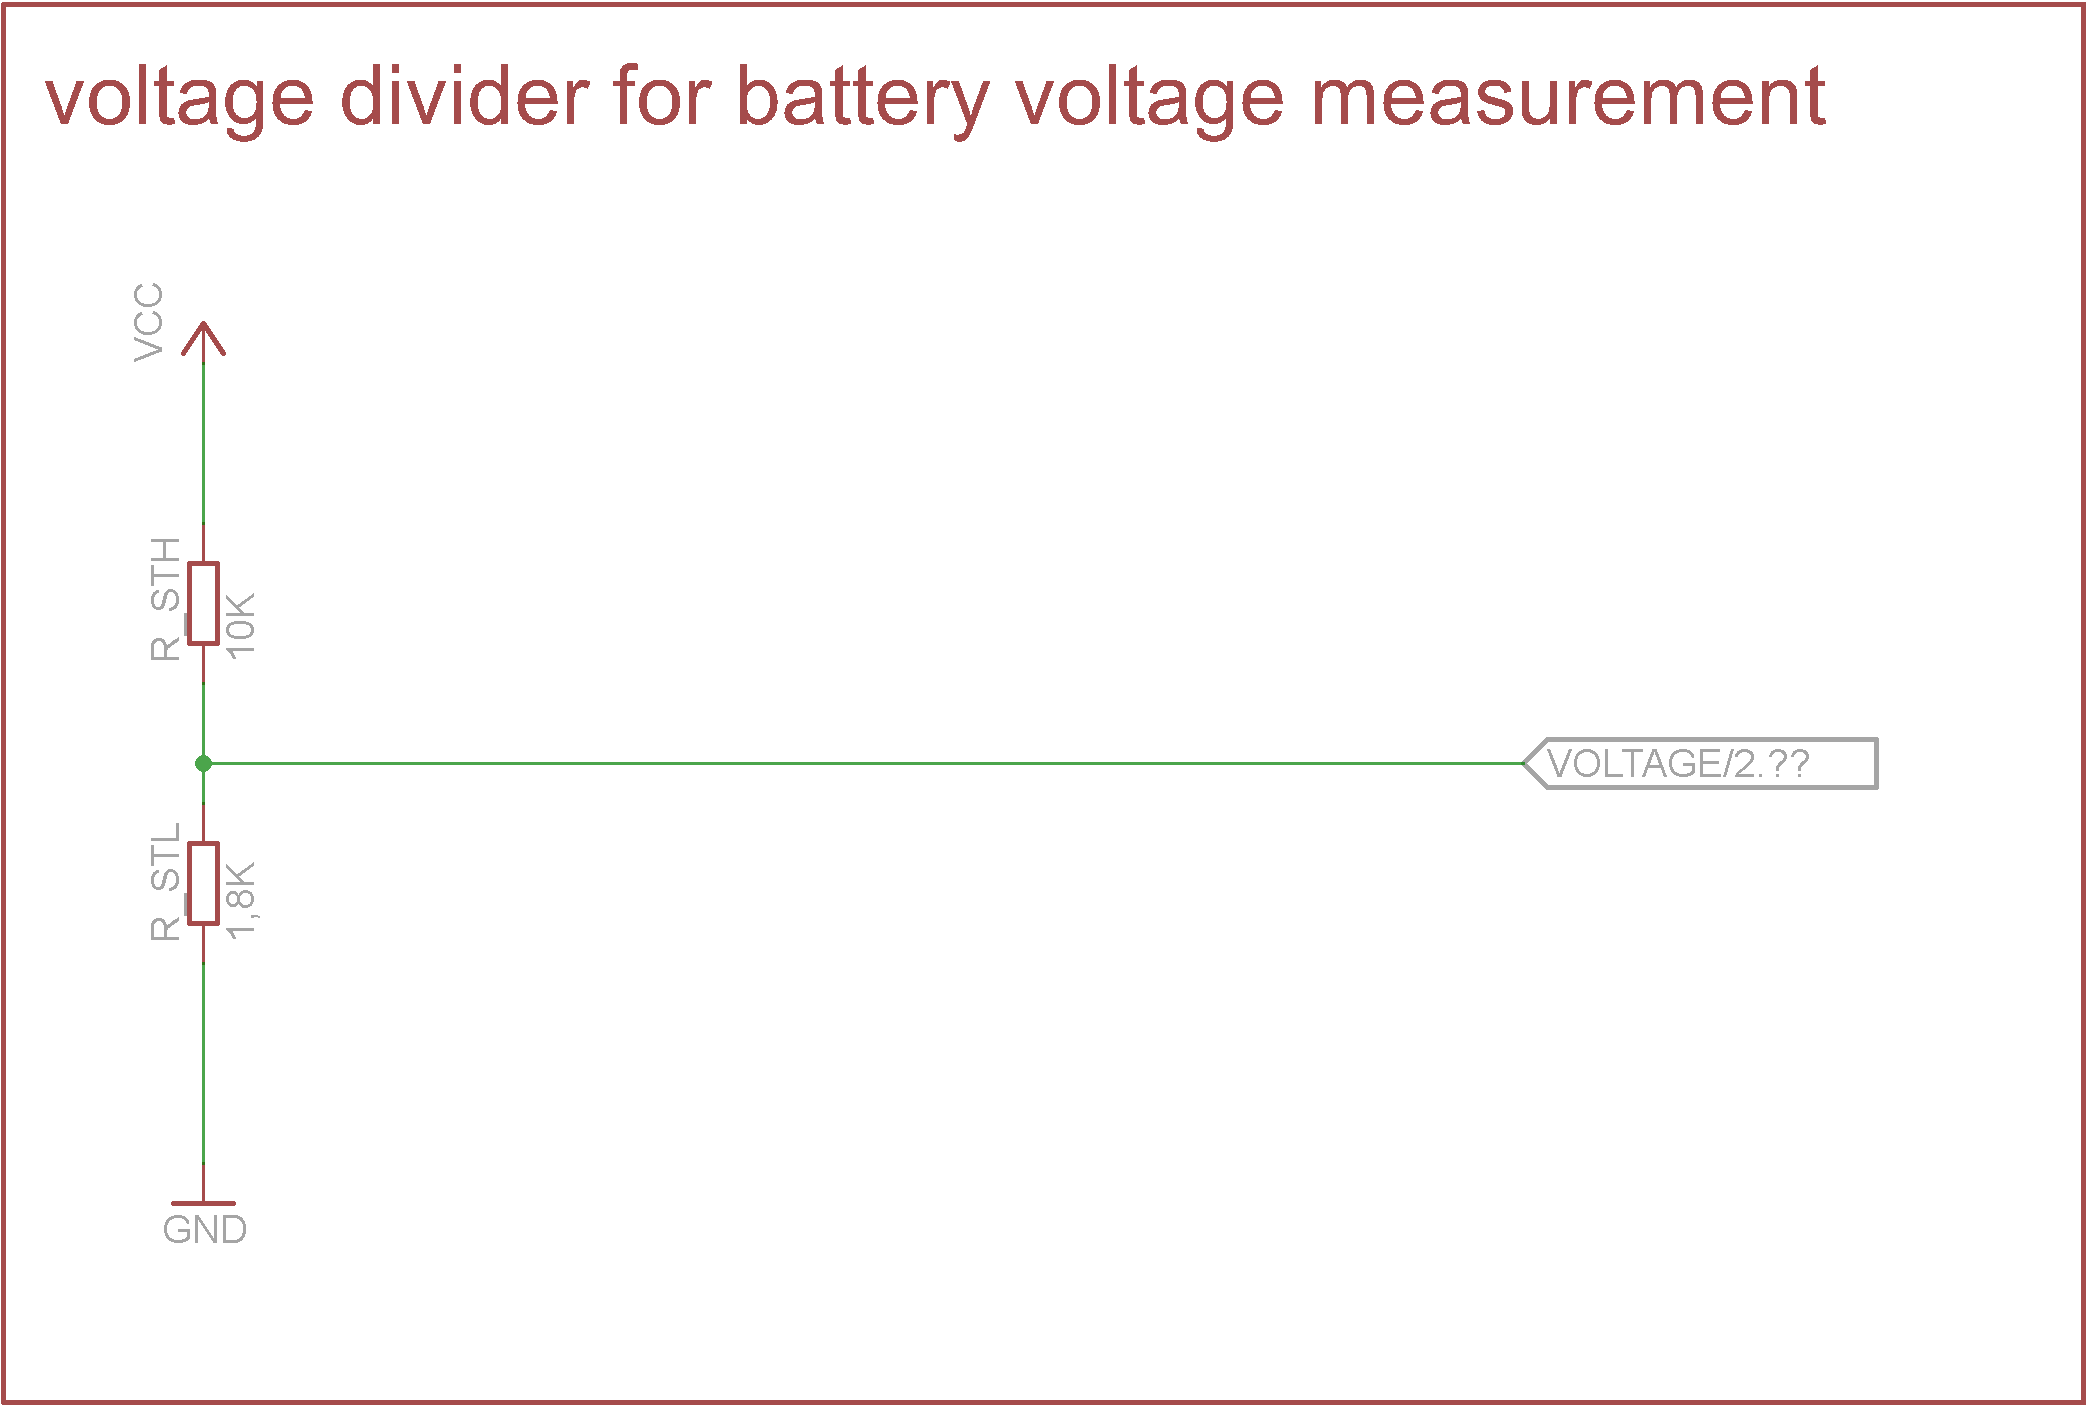
\includegraphics[width=\textwidth]{spannungsteiler.png}\\
\caption{Spannungsteiler zur Akkuspannungsmessung}%
\label{fig:Spannungsteiler}
\end{figure}

Da der Innenwiderstand des ADC sehr groß ist (\SI{100}{\milli\ohm}), kann der Spannungsteiler als unbelastet betrachtet werden. Damit ergibt sich das Teilungsverhältnis zu $\frac{R_{STL}}{R_{STH}+R_{STL}}=\num{0,153}$.
Die maximal messbare Akkuspannung beträgt dadurch $\frac{\SI{5}{\volt}}{\num{0,152}}=\SI{32,7}{\volt}$. Die Messung des Stroms gestaltet sich wesentlich aufwändiger und wird im Folgenden erläutert.


%\todo{Maximale Betiebsspannung ermitteln!!
%LM2678= 45 Volt
%Allegro= 50V
%Mosftes = 30V
%}


\subsection{Problem}

Die Messung des Motorstroms ist mit einem Problem behaftet, da der Motor über eine Pulsweitenmodulation angesteuert wird. Der Verlauf des Stroms ist pulsierend, abhängig von
der Frequenz und dem Tastgrad der Pulsweitenmodulation. In \cref{fig:pwm+i_0} zu erkennen ist der Verlauf des PWM Signals (obere Kurve) und des Stroms, welcher nach einer $1-e^t$ Funktion ansteigt.
Ohne weitere Filterung des Signals wäre eine extrem hohe Abtastfrequenz des ADC nötig, um den genauen Stromfluss zu messen. Da für eine Verbrauchsmessung 
der Mittelwert des Stroms interessant ist, kann dieser mit Hilfe eines Tiefpasses erzeugt werden.


\begin{figure}[H]
\centering
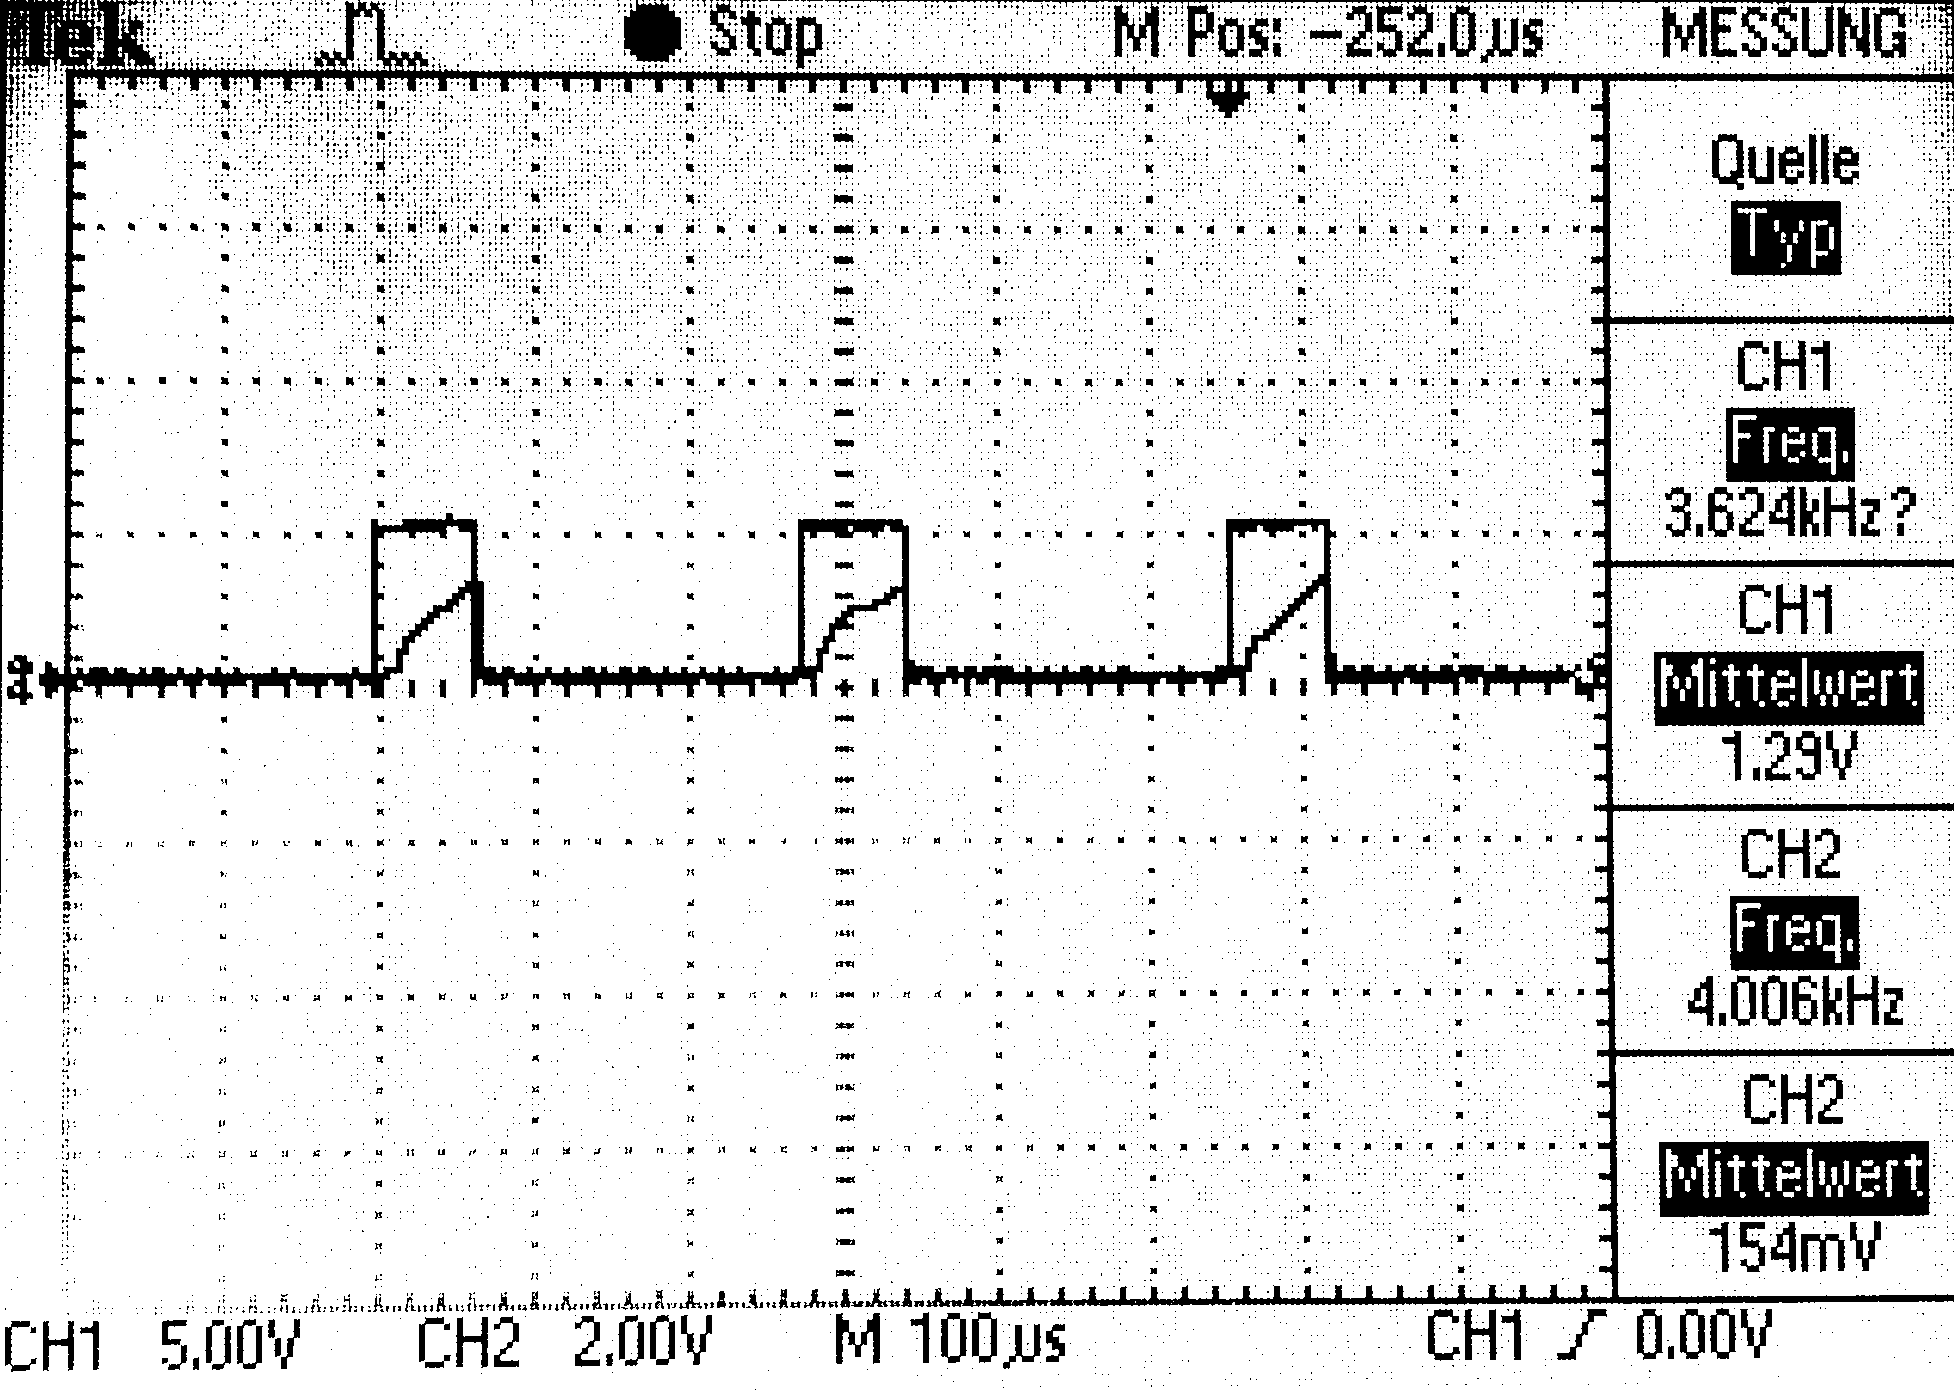
\includegraphics[width=.8\textwidth]{oszi.png}\\
\caption{Spannung am Shunt + PWM}%
\label{fig:pwm+i_0}
\end{figure}

Eine kostengünstige Variante den Strom zu messen ist den Spannungsabfall über einen Shuntwiderstand zu bestimmen. Die Größe des Shuntwiderstandes sollte nur so klein wie nötig gewählt werden.
Ein zu kleiner Shuntwiderstand benötigt einen starken Messverstärker, um das Signal auswerten zu können. Die Qualität und Genauigkeit dieses Signals nimmt allerdings mit steigender Verstärkung ab.

Nach kurzer Recherche wurde die Größe des Shuntwiderstands auf R2512(ca. \SI{6,35}{\milli\meter} x \SI{3,00}{\milli\meter}) begrenzt. Messshunts in dieser Größe gibt es problemlos bis zu einer Belastbarkeit von \SI{2}{\watt}. 
Bei einem maximalen Motorstrom von \SI{20}{\ampere} ergibt sich somit ein maximaler Spannungsabfall von \SI{100}{\milli\volt}. Nach dem Ohmschen Gesetz ergibt sich so eine Shunt-Größe von
$\frac{\SI{0,1}{\volt}}{\SI{20}{\ampere}}=\SI{0,005}{\ohm}$. Shuntwiderstände in der Größe sind problemlos zu bekommen.
Da es sich hier um eine Worst Case Rechnung handelt, wird der zusätzliche Widerstand des Shuntwiderstandes und der damit verringerte Strom bewusst ignoriert.

Der Shunt wird direkt unter der H-Brücke des Motortreibers gegen Masse geschaltet. So wird eine Messung gegen Masse durchgeführt. Die so über den Shuntwiderstand gemessene Spannung könnte 
dann über den ADC Eingang des Mikrocontrollers eingelesen werden. Vorher jedoch muss das Signal gefiltert und verstärkt werden.

\subsection{Anforderungen}
Die maximale Auflösung des Mikrocontrollers soll ausgenutzt werden. Der ADC des Mikrocontrollers arbeitet mit einer Auflösung von 10 Bit und einer 
Referenzspannung von \SI{5}{\volt}. Um die Auflösung des ADC auszunutzen muss das Signal, aufgrund des geringen Spannungsabfalls, verstärkt werden.

Als Anforderung ergibt sich außerdem, dass der maximale Ripple des Endsignals kleiner ist als der Quantisierungsfehler des ADC.
So ist es möglich auf eine zusätzliche digitale Filterung weitgehend zu verzichten.
Die kleinst mögliche zu erfassende Spannung des ADC beträgt $\frac{\SI{5}{\volt}}{2^{10}}=\SI{4,88}{\milli\volt}$.
Diesen Wert sollte der Ripple des Endsignales nicht überschreiten.
Aus einem möglichst kleinem Ripple resultiert eine möglichst hohe Filterordnung bzw. eine niedrige Grenzfrequenz.
Allerdings soll $U_{DC}$ einer Änderung des Mittelwertes, also einer Änderung des Tastverhältnisses, möglichst
schnell folgen. Diese Anforderung widerspricht der Vorherigen, so dass ein Kompromiss gefunden werden muss.

\subsection{Bestimmung des Filtertyps}
Da zum Verstärken des Signals aktive elektronische Elemente notwendig sind, z.B. ein Operationsverstärker, wird an dieser Stelle gleich ein aktiver Filter verwendet. 
Dieser gibt uns die Möglichkeit das Messsignal zu verstärken und gleichzeitig zu
filtern. Da das Signal im optimalen Fall eine Gleichspannung darstellt, müssen die hochfrequenten Anteile des Signales herausgefiltert werden. Dies geschieht 
mit Hilfe eines Tiefpasses. Es gibt im Grunde zwei übliche aktive Tiefpässe, den Tiefpass mit Mehrfachgegenkopplung und den Sallen-Key Filter. Ersterer verwendet
einen invertierenden Verstärker, dieser invertiert das Messsignal. Da der Mikrocontroller jedoch nur mit positiven Spannungen umgehen kann, müsste man hier mit einer 
negativen Referenzspannung arbeiten, was den Schaltungsaufwand unnötig vergrößern würde. Der Sallen-Key Tiefpass benutzt einen nicht invertierenden Verstärker, welcher diesen
Nachteil nicht hat. So dass ab dieser Stelle ein Sallen-Key Tiefpass entworfen wird.

\subsection{Die Filterschaltung}

Wie im vorherigen Abschnitt diskutiert, wird hier ein Sallen-Key Tiefpass entworfen. Zum Entwurf der Schaltung wurde Eagle genutzt.
Genutzt wird ein AD8628  Rail-to-Rail Operationsverstärker von Analog Devices, da dieser direkt an einer einzelnen 5V Spannung betrieben werden kann und
über hervorragende Eigenschaften verfügt \cite{ds-opv}. Die fertige Schaltung kann in \cref{fig:fschalt} betrachtet werden. Um Konflikte im Schaltplan zu vermeiden,
wurden den Variablen ein ``F'' vorangestellt.
\begin{figure}[H]
\centering
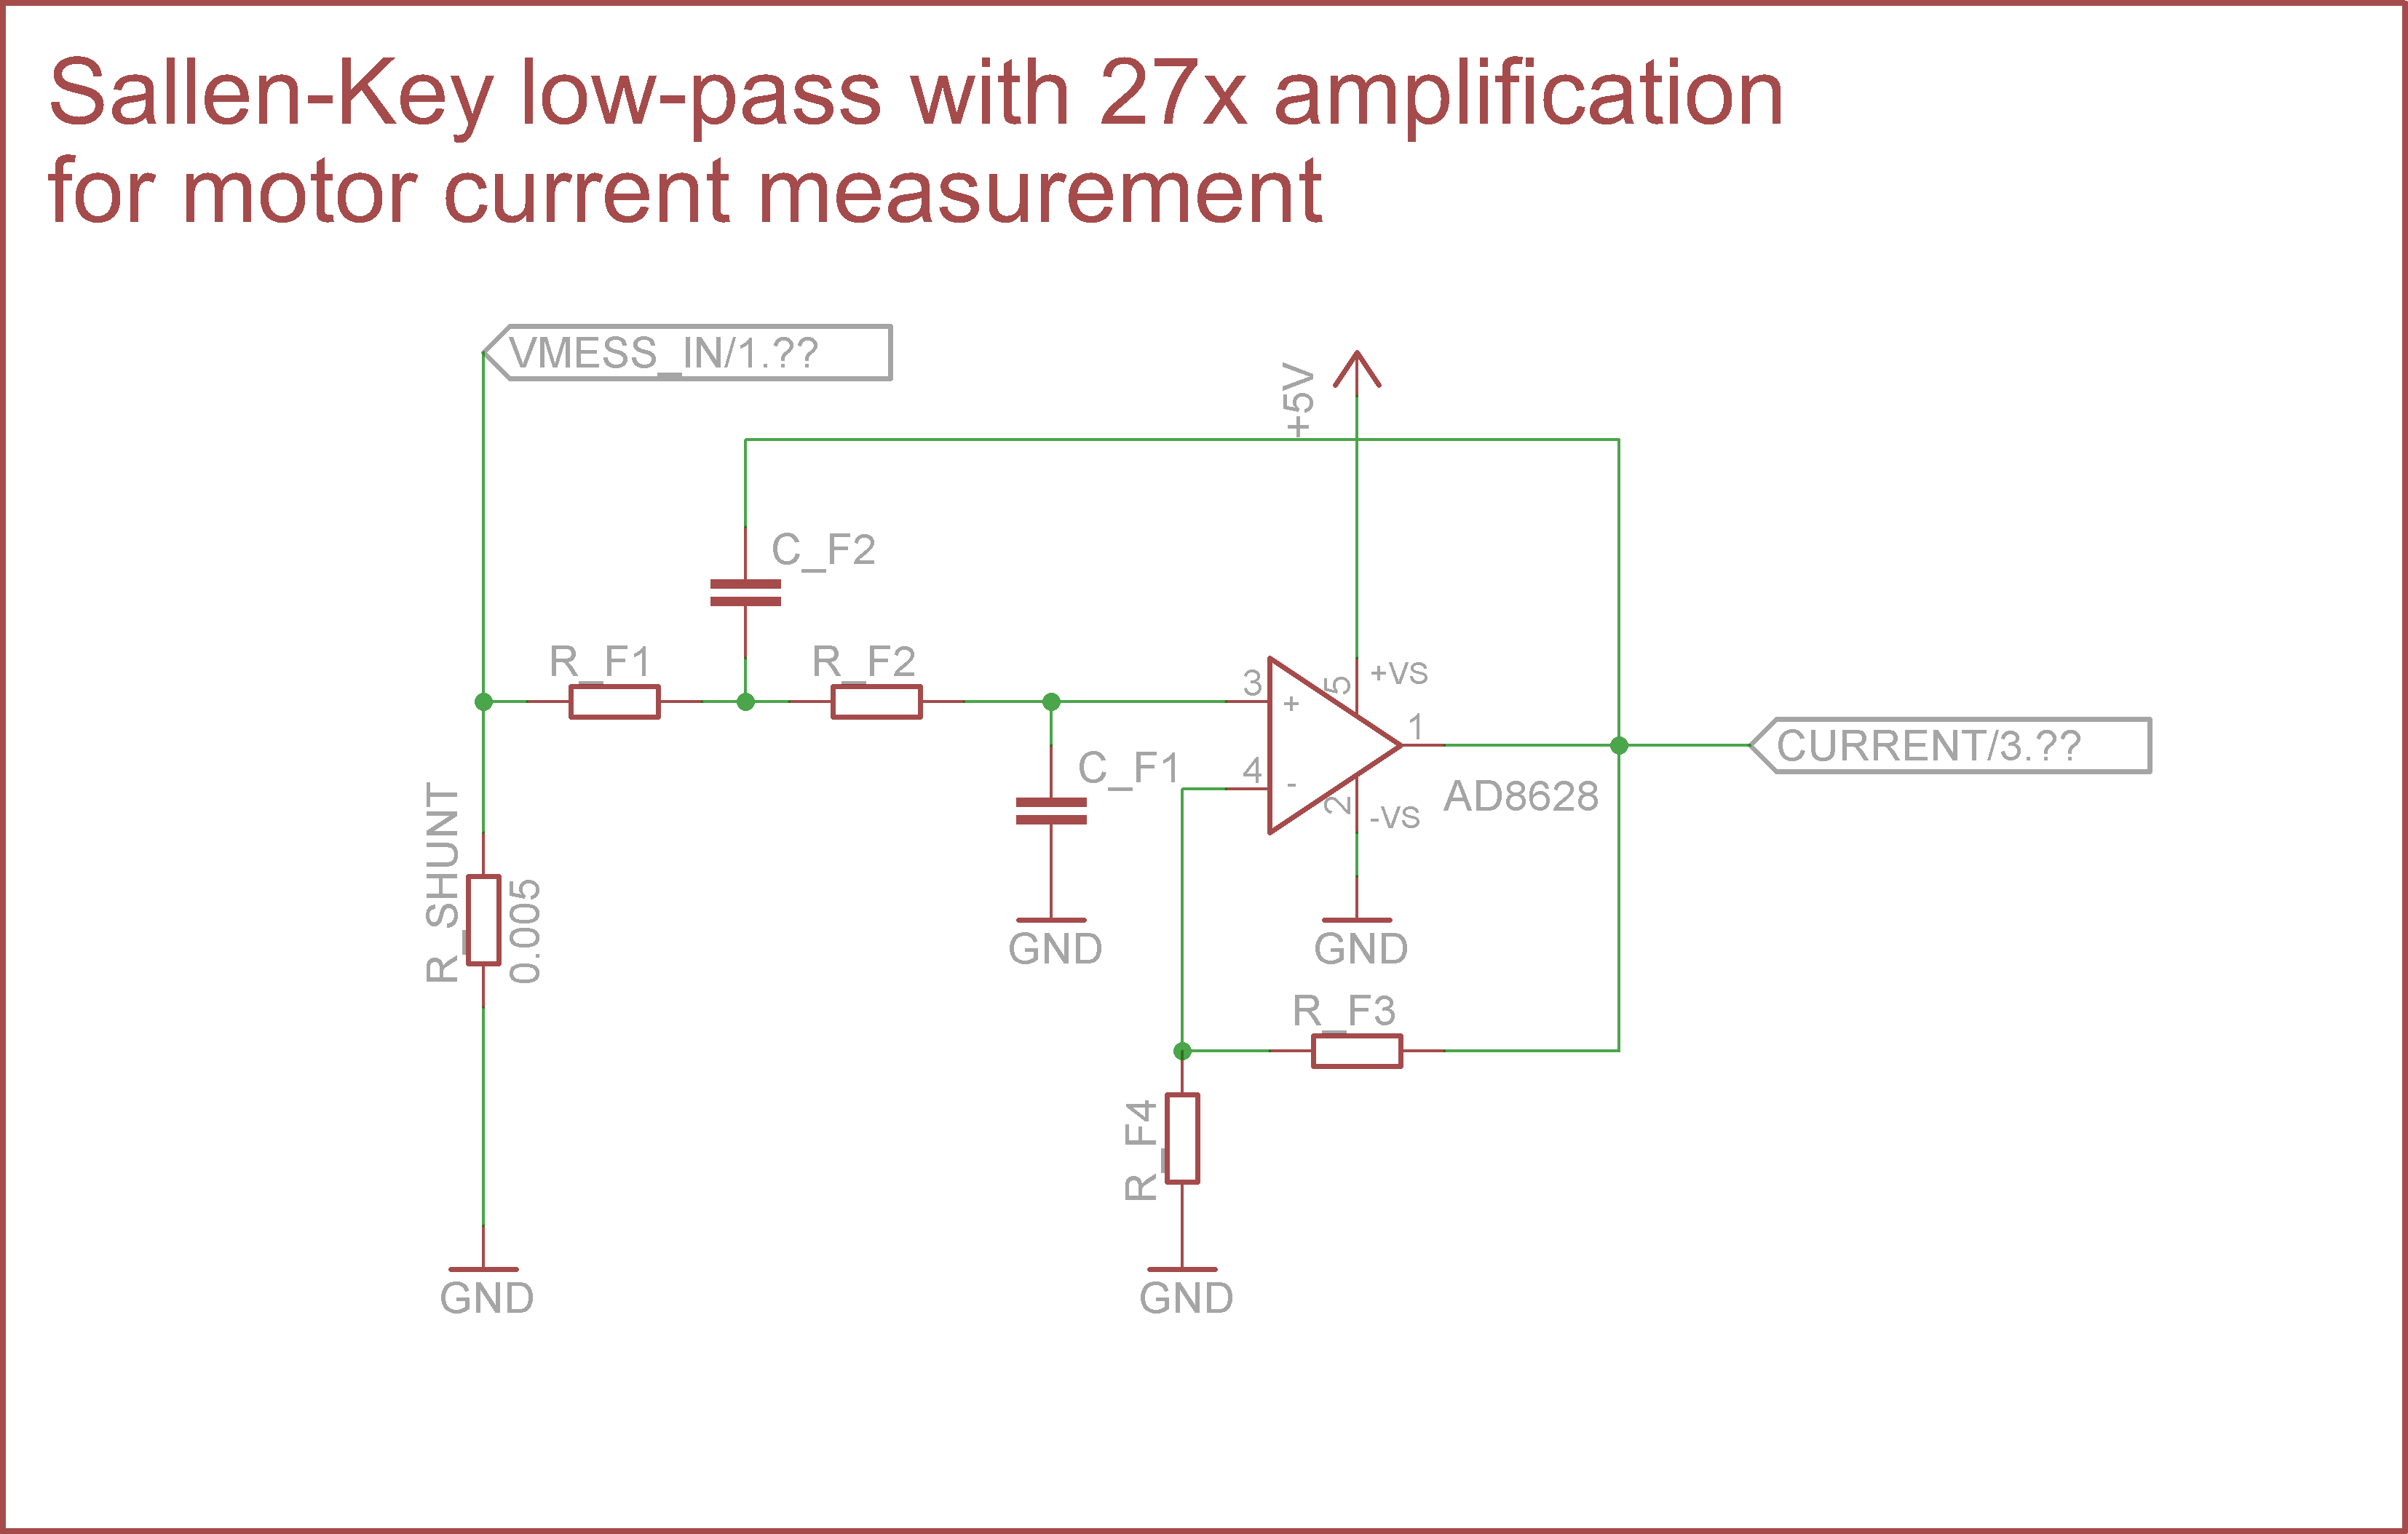
\includegraphics[width=\textwidth]{filter_schaltung.png}\\
\caption{Sallen-Key Tiefpass mit Shunt}%
\label{fig:fschalt}
\end{figure}



\subsection{Dimensionierung des Verstärkers}

In bisherigen Rechnungen wurde ein maximaler Spannungsabfall von \SI{100}{\milli\volt} am Shunt errechnet. Da der Messbereich des ADC voll ausgenutzt werden soll,
ist es nötig das Messsignal zu verstärken. Hierzu wird ein nicht-invertierender Verstärker genutzt. Da der Messbereich des ADC bis \SI{5}{\volt} reicht, wird hier eine 
50-fache Verstärkung angestrebt.

Die Beschaltung, welche den Verstärkungsfaktor des Sallen-Key Tiefpass festlegt, entspricht der eines nicht-invertierenden Verstärkers:

\begin{align*}
v &= 1 + \frac{R_{3}}{R_{4}}\\
50 &= 1 + \frac{R_{3}}{R_{4}}\\
49\cdot R_{4} &= R_{3}
\end{align*}
\\
Wobei $R_{F4} = \SI{47}{\kilo\ohm}$ und $R_{F3} = \SI{1}{\kilo\ohm}$  gewählt werden, was eine Ver\-stär\-kung von 48 ergibt. Die Größen sollten nicht zu klein gewählt werden, 
da der Operationsverstärkerausgang sonst zu stark belastet wird. Ein Gesamtwiderstand von \SI{5}{\kilo\ohm} resultiert stets in einem Stromverbrauch von unter \SI{1}{\milli\ampere} und ist
akzeptabel.


\subsection{Anforderungen an den Filter}

\begin{figure}[H]
\centering
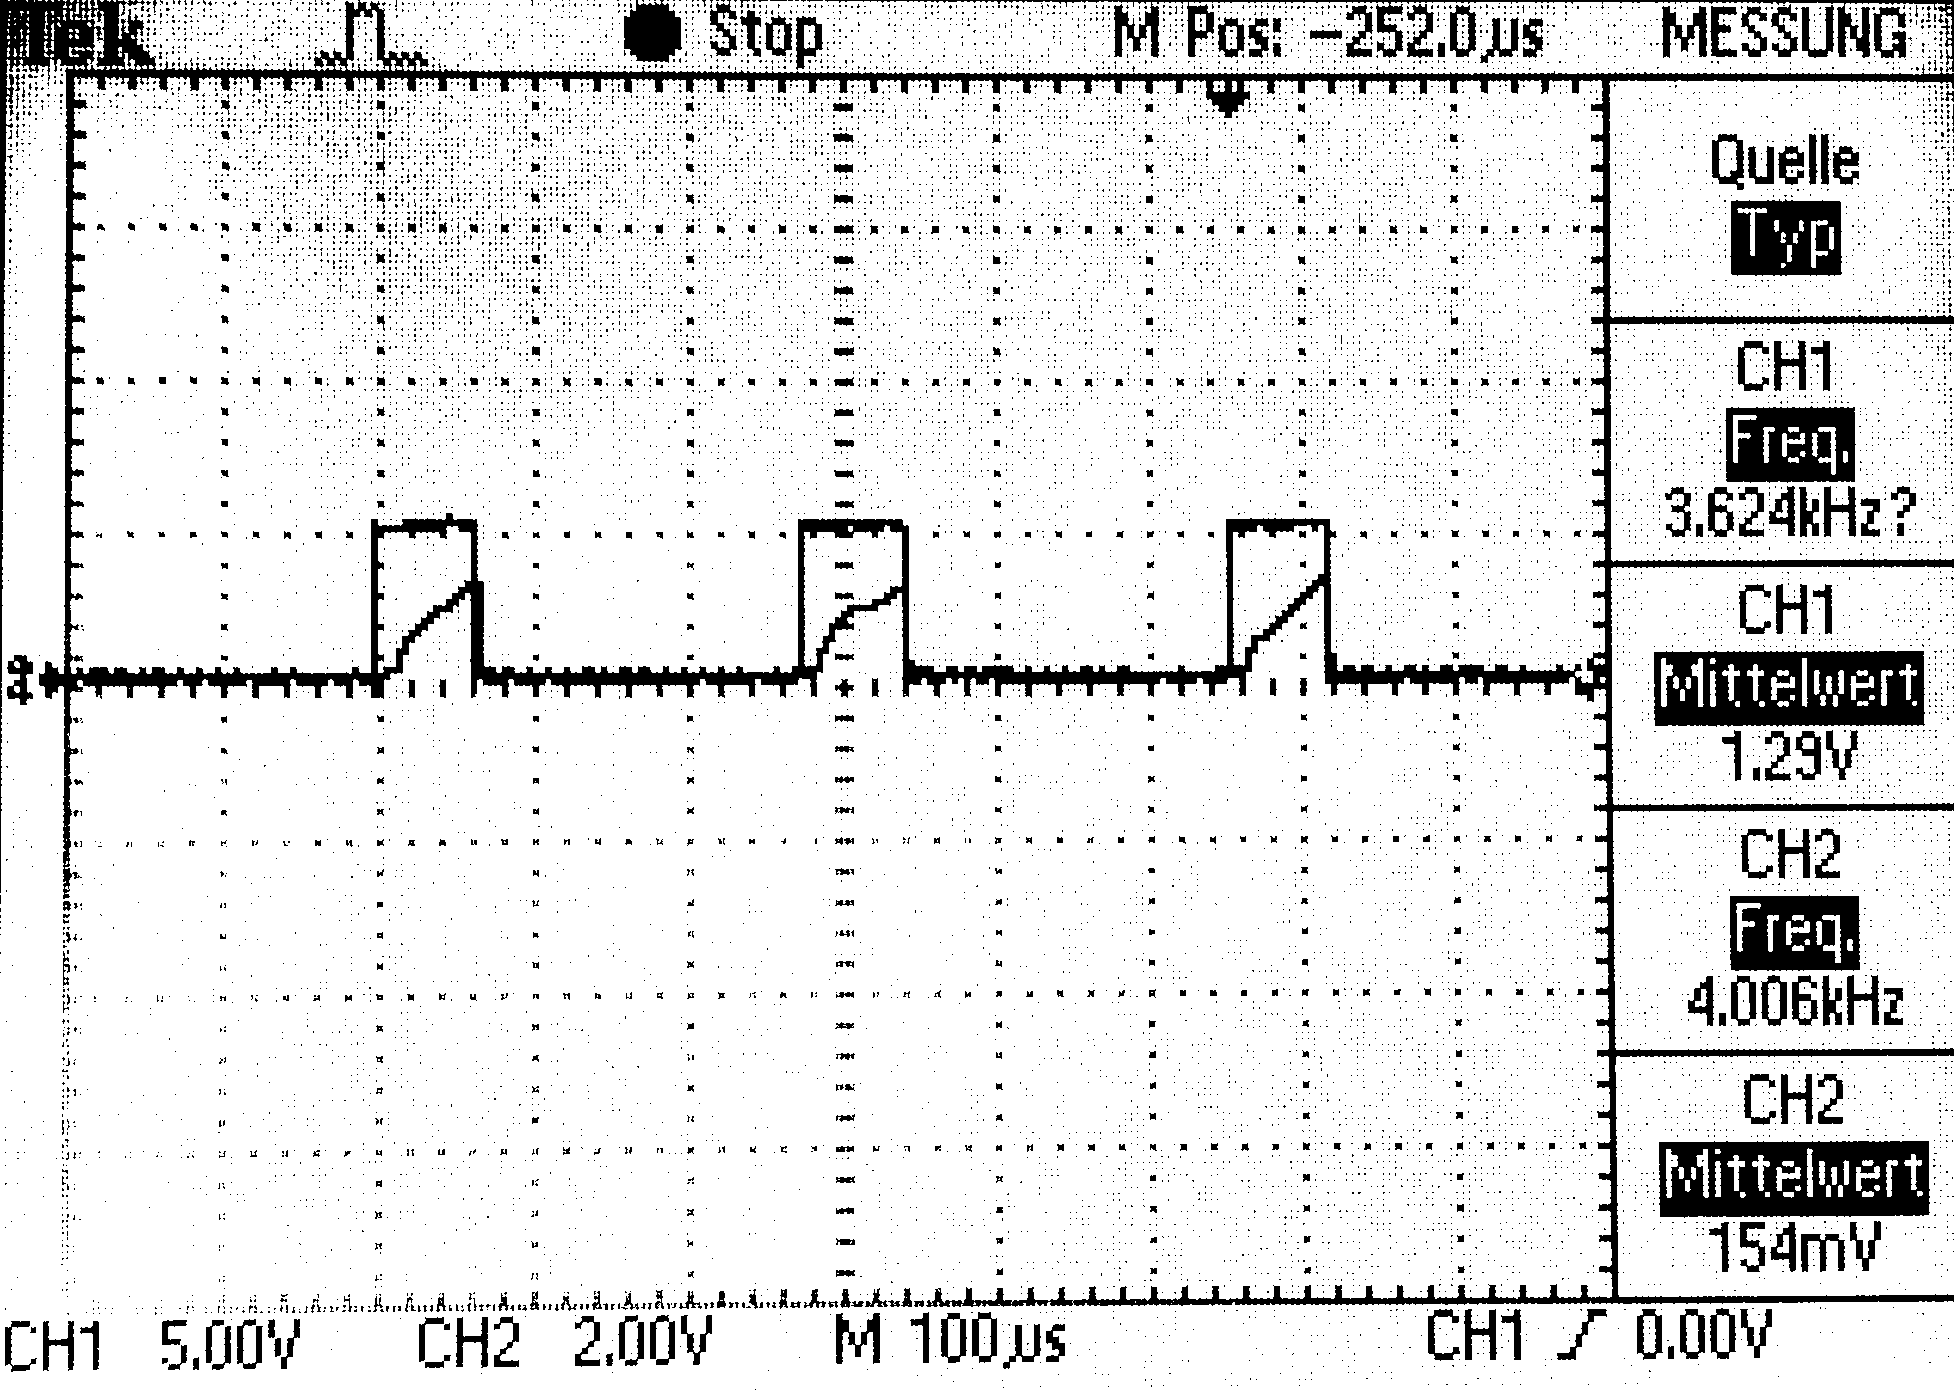
\includegraphics[width=.8\textwidth]{oszi.png}\\
\caption{Spannung am Shunt + PWM}%
\label{fig:pwm+i2}
\end{figure}

Da dem Messsignal wie in \cref{fig:pwm+i2} zu erkennen, die PWM Frequenz zu Grunde liegt, wird sich bei der Dimensionierung des Filters einer Idee nach \cite{Alter2008} bedient, nach der die maximale Amplitude des Ripple der Grundschwingung bei einem
Tastverhältnis von \num{0,5} ent\-spricht. Die Amplitude der Grundschwingung ergibt sich aus dem ersten Koeffizienten der Fourierreihe einer Rechteckschwingung.
\begin{align}
A_1 = K\cdot \frac{1}{\pi}[\sin(\pi p)-\sin(2\pi(1-\frac{p}{2}))]
\label{eq:ripple}
\end{align}
Wobei $p$ dem Tastverhältnis und $K$ der maximale Amplitude des Ursprungssignal entspricht \cite{Alter2008}. $K$ entspricht den errechneten \SI{100}{\milli\volt} multipliziert mit dem Verstärkungsfaktor 48, also \SI{4,8}{\volt}. 
Das Tastverhältnis $p$ wird zu 0,5
angenommen. Mit (\ref{eq:ripple}) ergibt sich für die Amplitude der Grundschwingung $ A_1 = K\cdot \frac{2}{\pi} = \SI{3,056}{\volt}$. $A_1$ soll auf $ < \SI{4,88}{\milli\volt}$ gedämpft werden.
Als Sperrfrequenz $\Omega_s $ wird hier die PWM Frequenz angesetzt. Für $H(\omega=2\pi f_{PWM})$ gilt also:

\begin{align}
H(\omega=2\pi f_{PWM}) \le \frac{\SI{4,88}{\milli\volt}}{\SI{3,056}{\volt}} \mathop{\hat{=}} 20\cdot\log(\frac{\SI{4,88}{\milli\volt}}{\SI{3,056}{\volt}})= \SI{-55,9}{\decibel}
\label{eq:daempfung}
\end{align}

Um die Komplexität der Schaltung gering zu halten, wird im Folgenden von den üblichen Konventionen zur Dimensionierung von Filtern abgewichen.
Statt eine fixe Grenzfrequenz festzulegen und die benötigte Filterordnung zu bestimmen, wird die Filterordnung vorgegeben und die Grenzfrequenz variiert.

\subsection{Filterentwurf}

\subsubsection{Bestimmung der Filtercharakteristik}

Die Charakteristik eins Filters entscheidet über seinen Frequenzgang. Es gibt viele dieser Filtercharakteristiken, eine Auswahl an häufig verwendeten Charakteristiken wird hier verglichen.

Der \emph{Butterworth}-Filter besitzt einen maximal flachen Verlauf des Frequenzganges im Durchlassbereich und eine monoton verlaufende Dämpfung im Sperrbereich.
Leider hat der Butterworth-Filter nur eine geringe Flankensteilheit im Sperrbereich (\SI{20}{\decibel}/Dekade pro Ordnung). Ein Butterworth-Filter 1. Ordnung entspricht einen  einfachen RC-Filter.

Der \emph{Tschebyscheff}-Filter hat eine höhere Flankensteilheit als der But\-ter\-worth-Filter, allerdings entsteht beim Tschebyscheff-Filter Welligkeit im Durchlassbereich,
welche mit höherer Ordnung zunimmt. Durch die Welligkeit im Durchlassbereich würde ein zusätzlicher Ripple im Signal entstehen, weshalb der Tschebyscheff-Filter nicht
für den geforderten Filter geeignet ist. 

Der \emph{Bessel-Filter} hat den Vorteil einer konstanten Gruppenlaufzeit, hat dafür aber eine noch geringere Flankensteilheit als der Butterworth-Filter.
Da eine konstante Gruppenlaufzeit für den geforderten Filter nicht von Vorteil ist, da das Endsignals einer Gleichspannung entsprechen sollte, ist der Butterworth-Filter
die bessere Wahl.


\subsubsection{Bestimmung der Grenzfrequenz}

Zur Bestimmung der Grenzfrequenz des Filters ist es nötig die PWM-Frequenz der Motoransteuerung zu kennen. Diese kann jedoch nur im Betrieb optimal bestimmt werden, da sie
auch von subjektiven Kriterien wie dem Motorgeräusch abhängt. Um den Filter trotzdem auslegen zu können wird sie auf \SI{3,9}{\kilo\hertz} festgelegt. Diese Frequenz
lässt sich im AVR durch den Phase Correct Modus mit einem Prescaler von 8 erreichen.

\begin{align*}
f_{PWM}=\frac{f_{CPU}}{Prescaler\cdot 2 \cdot 256} = \frac{\SI{16}{\mega\hertz}}{8 \cdot 2 \cdot 256 }=\SI{3906,25}{\hertz}
\end{align*}


\begin{figure}[H]
\centering
\begin{tikzpicture}
	\draw[->,thick] (0,0) -- (7.5,0) node[right] {$f[\text{Hz}]$};
	\draw[->,thick] (0,0) -- (0,3.3) node[above] {$a[\text{dB}]$};
	\draw (0,2.5)node[left] {$a_{\text{min}}$} (-0.1,2.5)--(2.9,2.5);
	\draw (0,1)node[left] {$a_{\text{max}}$};
	\def \bsp{(0,1)--(1,1)--(1,2.4)--(1,2.4)--(0,2.4)}
	\draw (-0.1,1)--(1,1)--(1,2.4) (1,0)node[below] {$f_g$};
	\pattern[pattern=north east lines] \bsp;
	\draw[dashed] (1,1) -- (1,-0.1);
	\def \bsd{(3,0) -- (3,2.5) -- (7,2.5) -- (7,0)}
	\pattern[pattern=north east lines] \bsd;
	\draw (3,0)node[below] {$f_s$} -- (3,2.5) -- (7,2.5);

\end{tikzpicture}
\caption{Tiefpass Toleranzfeld}%
\label{fig:analog}
\end{figure}



Für die Schaltung wird nun ein Sallen Key Tiefpass 2. Ordnung nach Butterworth entworfen. Die PWM-Frequenz $f_{PWM}$ beträgt \SI{3,9}{\kilo\hertz}.

Die Sperrfrequenz entspricht der PWM Frequenz, also der Frequenz der Grundschwingung. $\Omega$ entspricht der mit der Grenzfrequenz 
normierten Frequenz $\Omega=\frac{f}{f_g}$. Nach (\ref{eq:daempfung}) ergibt sich für \ref{fig:analog}

$f_s=f_{PWM}=\SI{3,9}{\kilo\hertz}$; $a_{min}=\SI{55,9}{\decibel}$ und $a_{max}$ wird auf einen üblichen Wert von \SI{3}{\decibel} festgelegt.







\begin{align}
n \ge \frac{\log{\sqrt{\frac{e^{2a_{min}}-1}{e^{2a_{max}}-1}}}}{\log{\Omega_s}}
\label{eq:butterworth}
\end{align}
Die Filterordnung nach Butterworth wird nach (\ref{eq:butterworth}) bestimmt\cite{AnalogFilter}. Umgestellt nach $\Omega_s$ ergibt sich:

\begin{align}
\Omega_s \le  \left(\frac{e^{2a_{min}}-1}{e^{2a_{max}}-1}\right)^{\frac{1}{2n}}
\end{align}



Für die Berechnung der Sperrfrequenz $\Omega_s$ müssen  $a_{min}$ und $a_{max}$ in Neper umgerechnet werden. Wobei:
\begin{align*}
\SI{1}{\decibel} =  \frac{\ln{10}}{20}\si{{\neper}} = \SI{0,115129255}{\neper}   
\end{align*}

Damit ergibt sich für $a_{min}=\SI{55,9}{\decibel}\cdot \frac{\ln{10}}{20}=\SI{6,45}{\neper}$ und für  $a_{max}=\SI{3}{\decibel}\cdot \frac{\ln{10}}{20}=\SI{0,345}{\neper}$. Die Filterordnung wird auf 2 festgelegt.
\begin{align}
\Omega_s \le  \left(\frac{e^{2\cdot\SI{6,45}{\neper} }-1}{e^{2\cdot \SI{0,345}{\neper}}-1}\right)^{\frac{1}{2n}}  = 35,8
\end{align}

Die Grenzfrequenz $f_g$ ergibt sich jetzt aus:

\begin{align}
\frac{f_s}{\Omega_s} \le \frac{\SI{3,9}{\kilo\hertz}}{35,8} = \SI{108,9}{\hertz}
\end{align}

\subsubsection{Filterentwurf}
Im vorherigen Abschnitt wurde berechnet, dass die Grenzfrequenz des Filters kleiner als \SI{108,9}{\hertz} sein muss.
Im Folgenden wird nun ein Sallen-Key Filter 2. Ordnung mit einer Grenzfrequenz von \SI{100}{\hertz} entworfen.
Die genaue Wahl der Grenzfrequenz ist hier nicht relevant da die realen Bauteile nicht in  allen Größen 
verfügbar sind und daher am Schluss variiert werden müssen, wodurch sich die Grenzfrequenz des Filters leicht ändert.


\subsubsection{Finaler Entwurf}



Betrachten wir das Polstellen-Nullstellendiagramm eines Butterworth Filters 2. Ordnung, wie in [\cref{fig:filter_polnul}]


\begin{figure}[H]
\centering
\begin{tikzpicture}
	\draw[->,thick] (-3,0) -- (3,0) node[right] {$\text{Re}$};
	\draw[->,thick] (0,-3) -- (0,3) node[above] {$\text{Im}$};
	\draw[dashed,red,very thin] (-3,2) -- (3,2);
	\draw[dashed,red,very thin] (-3,-2) -- (3,-2);
	\draw[dashed,red,very thin] (2,-3) -- (2,3);
	\draw[dashed,red,very thin] (-2,-3) -- (-2,3);
	\draw[dashed,blue,very thin] (0,0) circle (2);
	\coordinate (x) at (225:2); 
	\coordinate (y) at (135:2);
	\draw[very thin] (0,0) -- (y);
	\draw[red,thick] (x) -- +(0.1,0.1)  (x) -- +(-0.1,-0.1) (x) -- +(0.1,-0.1) (x) -- +(-0.1,0.1);
	\draw[red,thick] (y) -- +(0.1,0.1)  (y) -- +(-0.1,-0.1) (y) -- +(0.1,-0.1) (y) -- +(-0.1,0.1);
	\draw (2,0)node[below] {$1$};
	\draw (-2,0)node[below] {$-1$};
	\draw (0,2)node[left] {$1$};
	\draw (0,-2)node[left] {$-1$};
	\draw (0,-2)node[left] {$-1$};
	\draw (0,0) (135:1cm) arc (135:180:1cm);
	\draw (-0.6,0.3)node {$\delta$};
\end{tikzpicture}
\caption{Polstellen-Nullstellendiagramm, Butterworth 2. Ordnung}
\label{fig:filter_polnul}
\end{figure}



Charakteristisch für den Butterworth-Filter ist, dass sich die Polstellen auf einer Kreisbahn befinden. Auf die Grenzfrequenz normiert hat dieser beim Butterworth-Filter den Radius
eins. Bei einem Butterworth 2. Ordnung befinden sie sich genau bei $\delta=45^\circ$. Das Interessante am Polstellen-Nullstellendiagramm ist, dass sich Polfrequenz $\Omega_P$ und 
Polgüte $Q_P$ einfach ablesen lassen. Die Polfrequenz $\Omega_P$ ist der Betrag der normierten Polstelle, welcher beim Butterworth-Filter immer eins ist.
Die Polgüte ist abhängig von $\delta$ und ergibt sich zu: $Q_P=\frac{1}{2\cos{\delta}}$. Für den Butterworth-Filter ergeben sich also $Q_P=0,707$ und $\Omega_P=1$

Betrachten wir die Übertragungsfunktion eines Sallen-Key Tiefpasses 2. Ordnung \cite[S. 101]{Krucker2000}:

\begin{align*}
A(P)&=\frac{A_0}{1+\omega_g (R_2 C_1 + R_1 C_1 + R_1 C_2(1-A_0))P + \omega_g^2R_1 R_2 C_1C_2P^2}
\end{align*}

mit
\begin{align*}
A_0=1+\frac{R_6}{R_5}
\end{align*}


Die Bauteilwerte erhält man durch einen Koeffizientenvergleich mit der entnormierten
Übertragungsfunktion ($P=\frac{s}{\omega}$) eines Tiefpasses 2. Ordnung:

\begin{align*}
A(P)&=\frac{A_0}{1+\frac{1}{\omega_g\Omega_PQ_P}s+\frac{1}{\omega_g^2\Omega_P^2}s^2}
\end{align*}

Die Auflösung des Vergleiches ist mit vielen mathematischen Umformungen verbunden, deswegen wird hier auf eine
externe Quelle verwiesen \cite[S. 102]{Krucker2000}.
Nach dem Koeffizientenvergleich ergibt sich

\begin{align*}
C_1&<\frac{C_2\cdot(1+4Q^2_P(A_0-1))}{4Q^2_P}\\
R_1&=\frac{1}{2\omega_g\Omega_PQ_P} \cdot \frac{C_2\pm\sqrt{C_2^2-4Q^2_PC_2(C_1+C_2(1-A_0))}}{C_2(C_1-C_2(1-A_0))}   \\
R_2&=\frac{1}{2\omega_g\Omega_PQ_P} \cdot \frac{C_2\pm\sqrt{C_2^2-4Q^2_PC_2(C_1+C_2(1-A_0))}}{C_1C_2}  \\
Q_p&=\frac{\sqrt{R_1R_2C_1C_2}}{C1(R_1+R_2)+R_1C_2(1-A_0)}\\
\Omega_p&=\frac{1}{\omega_g\sqrt{R_1R_2C_1C_2}}
\end{align*}

Dabei sind immer nur die positiven, reellen Lösungen zu verwenden.


\subsubsection{Bestimmung der Bauteilwerte}

Um die Übersicht zu wahren wird die Berechnung der Bauteilwerte hier nur auszugsweise aufgeführt. Zur Erinnerung,
die gegebenen Werte sind $Q_P=0,707$ ; $\Omega_P=1$ ; $A_0=48$ und $\omega_g = 2 \cdot \pi \cdot \SI{100}{\hertz}$.
$A_0$ ist die Gleichspannungsverstärkung, sie beschreibt den gewünschten Verstärkungsfaktor der bereits in einem vorherigen
Abschnitt mit 48 bestimmt wurde. Die Berechnungen wurden mit Hilfe eines Python-Scriptes ausgeführt, dabei wurden verschiedene
Konfigurationen durchgerechnet. Hauptsächlich wurde dabei darauf geachtet, dass sich der Filter mit den vor Ort vorhandenen SMD-Bauteilen
aufbauen lässt.

In den Berechnungen fiel auf, dass bei steigender Größe der Kondensatoren die Größe der Widerstände sinkt. Da Widerstände auch in großen Größen vorhanden waren,
wurde für den frei wählbaren $C_2$ ein kleiner Wert von \SI{82}{\nano\farad} gewählt.

\begin{align*}
C_1&<\frac{C_2\cdot(1+4\cdot0,707^2_P(48-1))}{4\cdot0,707^2}\\
C_1&<3,90\mu F
\end{align*}

$C_1$ soll nur kleiner sein als \SI{3,9}{\micro\farad} und wird ebenfalls auf \SI{82}{\nano\farad} gesetzt.

\begin{align*}
B_1&=\frac{\SI{82}{\nano\farad}\pm\sqrt{\SI{82}{\nano\farad}^2-4\cdot0,707^2\cdot\SI{82}{\nano\farad}(\SI{82}{\nano\farad}+\SI{82}{\nano\farad}(1-48))}}{\SI{82}{\nano\farad}(\SI{82}{\nano\farad}-\SI{82}{\nano\farad}(1-48))}\\
R_1&=\frac{1}{2\cdot\SI{100}{\hertz}\cdot0,707} \cdot B_1\\
R_1&=[\SI{-3176}{\ohm},\SI{2579}{\ohm}]
\end{align*}


\begin{align*}
B_2=&\frac{\SI{82}{\nano\farad}\pm\sqrt{\SI{82}{\nano\farad}^2-4\cdot0,707^2\cdot\SI{82}{\nano\farad}(\SI{82}{\nano\farad}+\SI{82}{\nano\farad}(1-48))}}{\SI{82}{\nano\farad}^2}\\
R_2&=\frac{1}{2\cdot\SI{100}{\hertz}\cdot0,707} \cdot B_2\\
R_2&=[\SI{146079}{\ohm},\SI{-118626}{\ohm}]
\end{align*}

Da nur positive Werte genutzt werden, ergeben sich die Bauteilwerte nun zu:
\begin{align*}
C_1&=\SI{82}{\nano\farad}\\
C_2&=\SI{82}{\nano\farad}\\
R_1&=\SI{2579}{\ohm}\\
R_2&=\SI{146079}{\ohm}
\end{align*}

In der folgenden Abbildung ist das Ergebnis der Simulation zu sehen. An der Abbildung leider nicht gut zu erkennen,
liegt der \SI{-3}{\decibel} Punkt genau bei \SI{100}{\hertz}. Die Frequenzachse des Diagrammes geht genau bis \SI{3,9}{\kilo\hertz}. 
Es ist eine Verstärkung von 48 des Ursprungssignals gewünscht. Diese Verstärkung wird mit \SI{33,6}{\decibel} bei \SI{10}{\hertz}, erreicht.
\begin{align*}
20\cdot\log{48}=\SI{-33,6}{\decibel}
\end{align*}

Bei \SI{3,9}{\kilo\hertz} erreicht der Filter eine Dämpfung von \SI{-30,1}{\decibel}. Zusammen mit der Verstärkung von \SI{33,6}{\decibel} des Eingangssignals 
wird das bereits verstärkte Signal also um \SI{63,7}{\decibel} gedämpft. Gefordert waren hier \SI{55,9}{\decibel}, so dass der Filter den geforderten Wert übersteigt, was an der niedrigeren Grenzfrequenz von \SI{100}{\hertz} statt \SI{108,9}{\hertz} liegt.

%%Verstärkung: 33,6dB gewünscht:
%%20*log(1/48)=-33,6

%%dämpfung bei 3,9Khz = 30,7dB
%% 33,6+30,1 =63,7 gewüncht: 55,9
%% Grenzfreqeunz = 100Hz (-3db)
\begin{figure}[H]
\centering
\begin{gnuplot}[terminal=pdf, scale=0.94]
  set nokey 
  set xrange [10:3900]
  set xlabel 'Frequenz in [Hz]'
  set ylabel 'Verstärkung in [dB]'
  set logscale x 10
  plot 'Simulation/Filter_original_frequenzgang.csv' with line
\end{gnuplot}
\caption{Frequenzgang des berechneten Filters}
\label{plott:filter_freq}
\end{figure}

Leider kann ein solcher Filter nur mit erheblichen Aufwendungen gebaut werden, da es keine fertigen Widerstände in den Größen $\SI{2579}{\ohm}\\$ und $\SI{146079}{\ohm}$ gibt. 
Da jedoch alle Widerstände der E12 Reihe vor Ort vorhanden sind, werden die realen Werte wie folgt gewählt: $R_1=\SI{2,7}{\kilo\ohm}\\ R_2=\SI{150}{\kilo\ohm}$, da sie den nächsten Größen in der E12 Reihe entsprechen.


In der folgenden Abbildung ist die Simulation des Filters mit den realen Bauteilwerten(blau) im Vergleich zum idealen Filter(rot) zu sehen.
Die Grenzfrequenz des Filters (\SI{-3}{\decibel}) liegt diesmal mit \SI{104}{\hertz} etwas über den ursprünglichen \SI{100}{\hertz}. Da wir die Werte von $R_5$ und $R_6$ nicht verändert haben, 
liegt die Verstärkung bei \SI{10}{\hertz} immer noch bei exakt \SI{33,6}{\decibel}. Bei \SI{3,9}{\kilo\hertz}, im Diagramm gut zu erkennen wird trotz der höheren Grenzfrequenz eine höhere Dämpfung als vorher erreicht.
Diese liegt bei \SI{33,7}{\decibel}. Daran kann man erkennen, dass es sich nicht mehr um einen idealen Butterworth-Filter handelt. 

%%Verstärkung: 33,6dB gewünscht:
%%20*log(1/48)=-33,6

%%dämpfung bei 3,9Khz = 30,7dB
%% 33,6+30,7 =64,3 gewüncht: 55,9
%% Grenzfreqeunz = 104Hz (-3db)
\begin{figure}[H]
\centering
\begin{gnuplot}[terminal=pdf, scale=0.94]
  set xrange [10:3900]
  set xlabel 'Frequenz in [Hz]'
  set ylabel 'Verstärkung in [dB]'
  set logscale x 10
  
  plot 'Simulation/Filter_original_frequenzgang.csv' with line linecolor rgb "red" title "Ideal", 'Simulation/Filter_real_frequenzgang.csv' with line linecolor rgb "blue" title "Real"
\end{gnuplot}
\caption{Frequenzgang des berechneten Filters mit finalen Bauteilwerten}
\label{plott:filter_freq_real}
\end{figure}

In der folgenden \ref{plott:filter_sprungantwort} ist 
die Antwort des Filters auf ein Rechtecksignal mit \SI{3,9}{\kilo\hertz}, einem Tastverhältnis von 0,5 und einer Amplitude von \SI{50}{\milli\volt} zu sehen. Das Überschwingen im Bereich
von \SI{7}{\milli\second} ist charakteristisch für den Butterworth-Filter und wirkt sich negativ auf die Messung des Stroms aus. Allerdings werden solch große Sprünge in der Praxis nicht auftreten,
da der Strom durch die große Induktivität des Motors nur langsam ansteigt.
\begin{figure}[H]
\centering
\begin{gnuplot}[terminal=pdf, scale=0.94]
  set nokey 
  set yrange [0:3]
  set xlabel 'Zeit in [s]'
  set ylabel 'Spannung in [V]'
  plot 'Simulation/Filter_real_time.csv' with line
\end{gnuplot}
\caption{Sprungantwort des Filters}
\label{plott:filter_sprungantwort}
\end{figure}


Die in \ref{plott:ripple} gut zu erkennende Restwelligkeit (Ripple) beträgt \SI{3,36}{\milli\volt} und liegt damit deutlich unter den geforderten \SI{4,88}{\milli\volt}. 
Als Eingangssignal dient hier ein Rechtecksignal mit \SI{3,9}{\kilo\hertz} und einem Tastverhältnis von 0,5, die Amplitude liegt bei \SI{50}{\milli\volt}. 
Die Tatsache, dass das Signal \SI{240}{\milli\volt} über den rechnerischen \SI{2,40}{\volt}  ($\SI{0,5}{\volt} \cdot 48 $) liegt, rührt daher, dass LT-Spice die Steig- und Fallzeiten in den low-Bereich des Rechtecksignals legt, 
wodurch der Mittelwert des Signals bei \SI{2,64}{\volt} liegt.
 
%% Ripple: 0,003358
%% zu hoher Spannungswert durch Steig und Fallzeiten im low bereich des Rechtecksignals
\begin{figure}[H]
\centering
\begin{gnuplot}[terminal=pdf, scale=0.94]
  set nokey 
  set xrange [0.03:0.04]
  set yrange [2.62:2.66]
  set xlabel 'Zeit in [s]'
  set ylabel 'Spannung in [V]'
  plot 'Simulation/Filter_real_time.csv' with line
\end{gnuplot}
\caption{Restwelligkeit des Filters}
\label{plott:ripple}
\end{figure}

Da der berechnete Filter den Anforderungen bestens genügt, wird dieser in die Schaltung übernommen.


\section{Beleuchtung}
Die einfachste Möglichkeit eine Beleuchtung am Auto zu realisieren sind Leuchtdioden, welche in allen erdenklichen Farben zu bekommen sind. Weiter Vorteile
sind ihre Energieeffizienz und günstigen Preise. LEDs stellen zudem keine großen Anforderungen an die Energieversorgung.

Das Hauptproblem bei der Integration von vielen LEDs ist die Verkabelung. Eine große Erleichterung bei der Integration sind 
LED-Streifen. Diese LED-Streifen gibt es in vielen Ausführungen. Für diese Arbeit interessant sind allerdings nur jene Vertreter, welche die Ansteuerung
jeder einzelnen LED zulassen. Die LED-Streifen mit Controllern von ``Worldsemi'' sind hierbei die prominentesten Vertreter. Zu erwähnen wären hierbei die Modelle
WS2801, WS2811 und WS2812. Der WS2812 ist dabei nahezu identisch mit dem WS2811 mit dem Unterschied, dass der WS2812 bereits in eine RGB-LED integriert ist.
Im Unterschied zum WS2801 werden die beiden durch eine einzige Signalleitung mit fixem Takt angesteuert, so dass hier eine separate Taktleitung entfällt.

Der Nachteil an dieser Methode ist, dass das Timing genau eingehalten werden muss, um die Daten korrekt zu übertragen. Wie in \cref{fig:led_cascade} werden die 
LEDs kaskadiert. Die Daten werden dann durch die LEDs geschoben.

\begin{figure}[H]
\centering
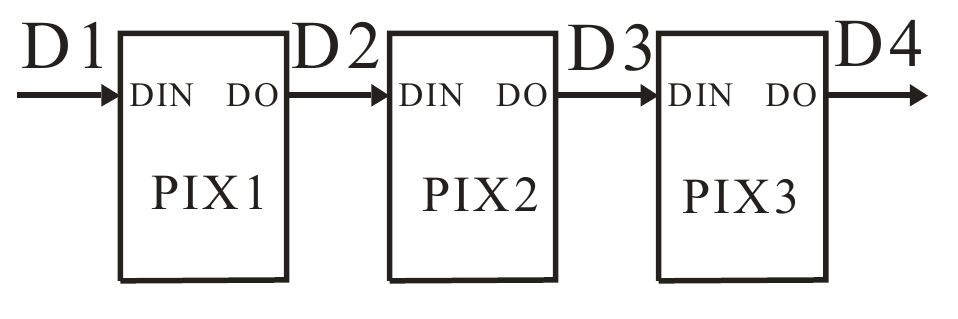
\includegraphics[width=.8\textwidth]{led_cascade.png}\\
\caption{Kaskadierung der LEDs \cite{ds-WS2812}}%
\label{fig:led_cascade}
\end{figure}

Um die Beleuchtung am Auto zu realisieren, werden LEDs mit WS2812 genutzt. Da die LEDs an einem beliebigen
Eingang des AVR-Mikro\-con\-trol\-lers angeschlossen werden können, wird der LED-Streifen an Pin PA5 angeschlossen. Da das Timing 
exakt eingehalten werden muss, ist die Software zur Ansteuerung in Assembler geschrieben.

Die LEDs werden wie folgt angesteuert:\\
Jede LED wird mit einem 24Bit Datenwort angesprochen, welches die Helligkeitsstufen für jede der drei Grundfarben enthält. 
Die Reihenfolge der Daten ist dabei grün, rot und dann blau. Das höchstwertige Bit wird zuerst übertragen.
Die Daten werden ohne Pause gesendet, bis alle LEDs im Strang die nötigen Daten erhalten haben. Nach jeder Übertragung muss eine Pause von mindestens \SI{50}{\micro\second} eingehalten
werden, damit die LEDs die Daten übernehmen. Die einzelnen Bits der Übertragung sind dabei folgendermaßen codiert:

\begin{figure}[H]
\centering
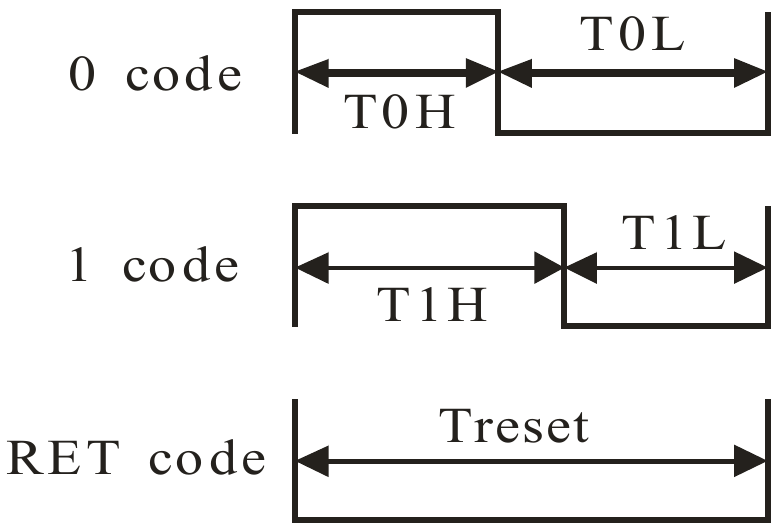
\includegraphics[width=.5\textwidth]{led_timing.png}\\
\caption{Codierung des LED Signals \cite{ds-WS2812}}%
\label{fig:led_timing}
\end{figure}

Die genauen Signallängen können \cref{tab:led_timing} entnommen werden.

\begin{table}[H]
  \centering
  \begin{tabularx}{\textwidth}{|r|X|r|r|}
    \hline
    Abschnitt & Beschreibung & Dauer & Abweichung \\ \hline
    T0H & 0 Code, high Zeit & $\SI{0,35}{\micro\second}$ & \textpm \SI{150}{\nano\second}\\ \hline
    T1H & 1 Code, high Zeit & $\SI{0,7}{\micro\second}$ & \textpm \SI{150}{\nano\second}\\ \hline
    T0L & 0 Code, low Zeit & $\SI{0,8}{\micro\second}$ & \textpm \SI{150}{\nano\second}\\ \hline
    T1L & 0 Code, low Zeit & $\SI{0,6}{\micro\second}$ & \textpm \SI{150}{\nano\second}\\ \hline
    RES & Reset Code, low Zeit & über $\SI{50}{\micro\second}$ & \\ \hline
  \end{tabularx}
  \caption{Signallängen}%
  \label{tab:led_timing}
\end{table}




\section{Distanzsensoren}

 
\subsection{Messprinzip}
Die ausgewählten Sensoren der Sharp GP2D Reihe basieren auf einer optischen Abstandsmessung, genauer der optischen Abstandsmessung durch Triangulation.
Bei der optische Abstandsmessung durch Triangulation projiziert ein Projektor einen Lichtpunkt auf das Messobjekt [\ref{fig:lasertriangulation}]. Ein optischer
Sensor misst dann den Winkel des vom Messobjekt reflektierten Lichts. Durch Triangulation kann dann durch den fest definierten Abstand des optischen
Sensors von der Lichtquelle die Entfernung zum Objekt berechnet werden. \cite{Hugenschmidt2007}. In \cref{fig:lasertriangulation} ist
dieses Prinzip veranschaulicht.
\begin{figure}[H]
\centering
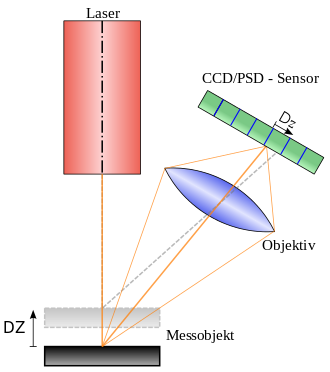
\includegraphics[width=.5\textwidth]{lasertriangulation.png}\\
\caption{Prinzip der Lasertriangulation \cite{lasertriangulation}}%
\label{fig:lasertriangulation}
\end{figure}

Vorteile des Messprinzips:
Da es sich um eine rein trigonometrische Messung handelt, kann sie zur kontinuierlichen Messung von beweglichen Objekten verwendet werden.
Außerdem besitzen Sensoren nach diesem Prinzip einen kleinen Messfleck.

Nachteile:
Die Messung ist stark von der Oberfläche des Messobjektes abhängig, spiegelnde Oberflächen stellen ein großes Problem dar.
In staubigen oder nebligen Umgebungen wird das Licht möglicherweise zu stark gestreut, so dass eine korrekte Messung nicht möglich ist.

\subsection{Probleme der GP2D Sensoren}
Die Sensoren verfügen über einen analogen Ausgang. Bei analogen Signalen ist generell mit Störungen zu rechnen. Die GP2D Sensoren scheinen
hohe Anforderungen an die Energieversorgung zu stellen. Hier ist eine Entstörung mittels Kondensator vonnöten, da im Messsignal sonst große Spikes
entstehen, wie in \cref{fig:IR_spikes} zu sehen.

\begin{figure}[H]
\centering
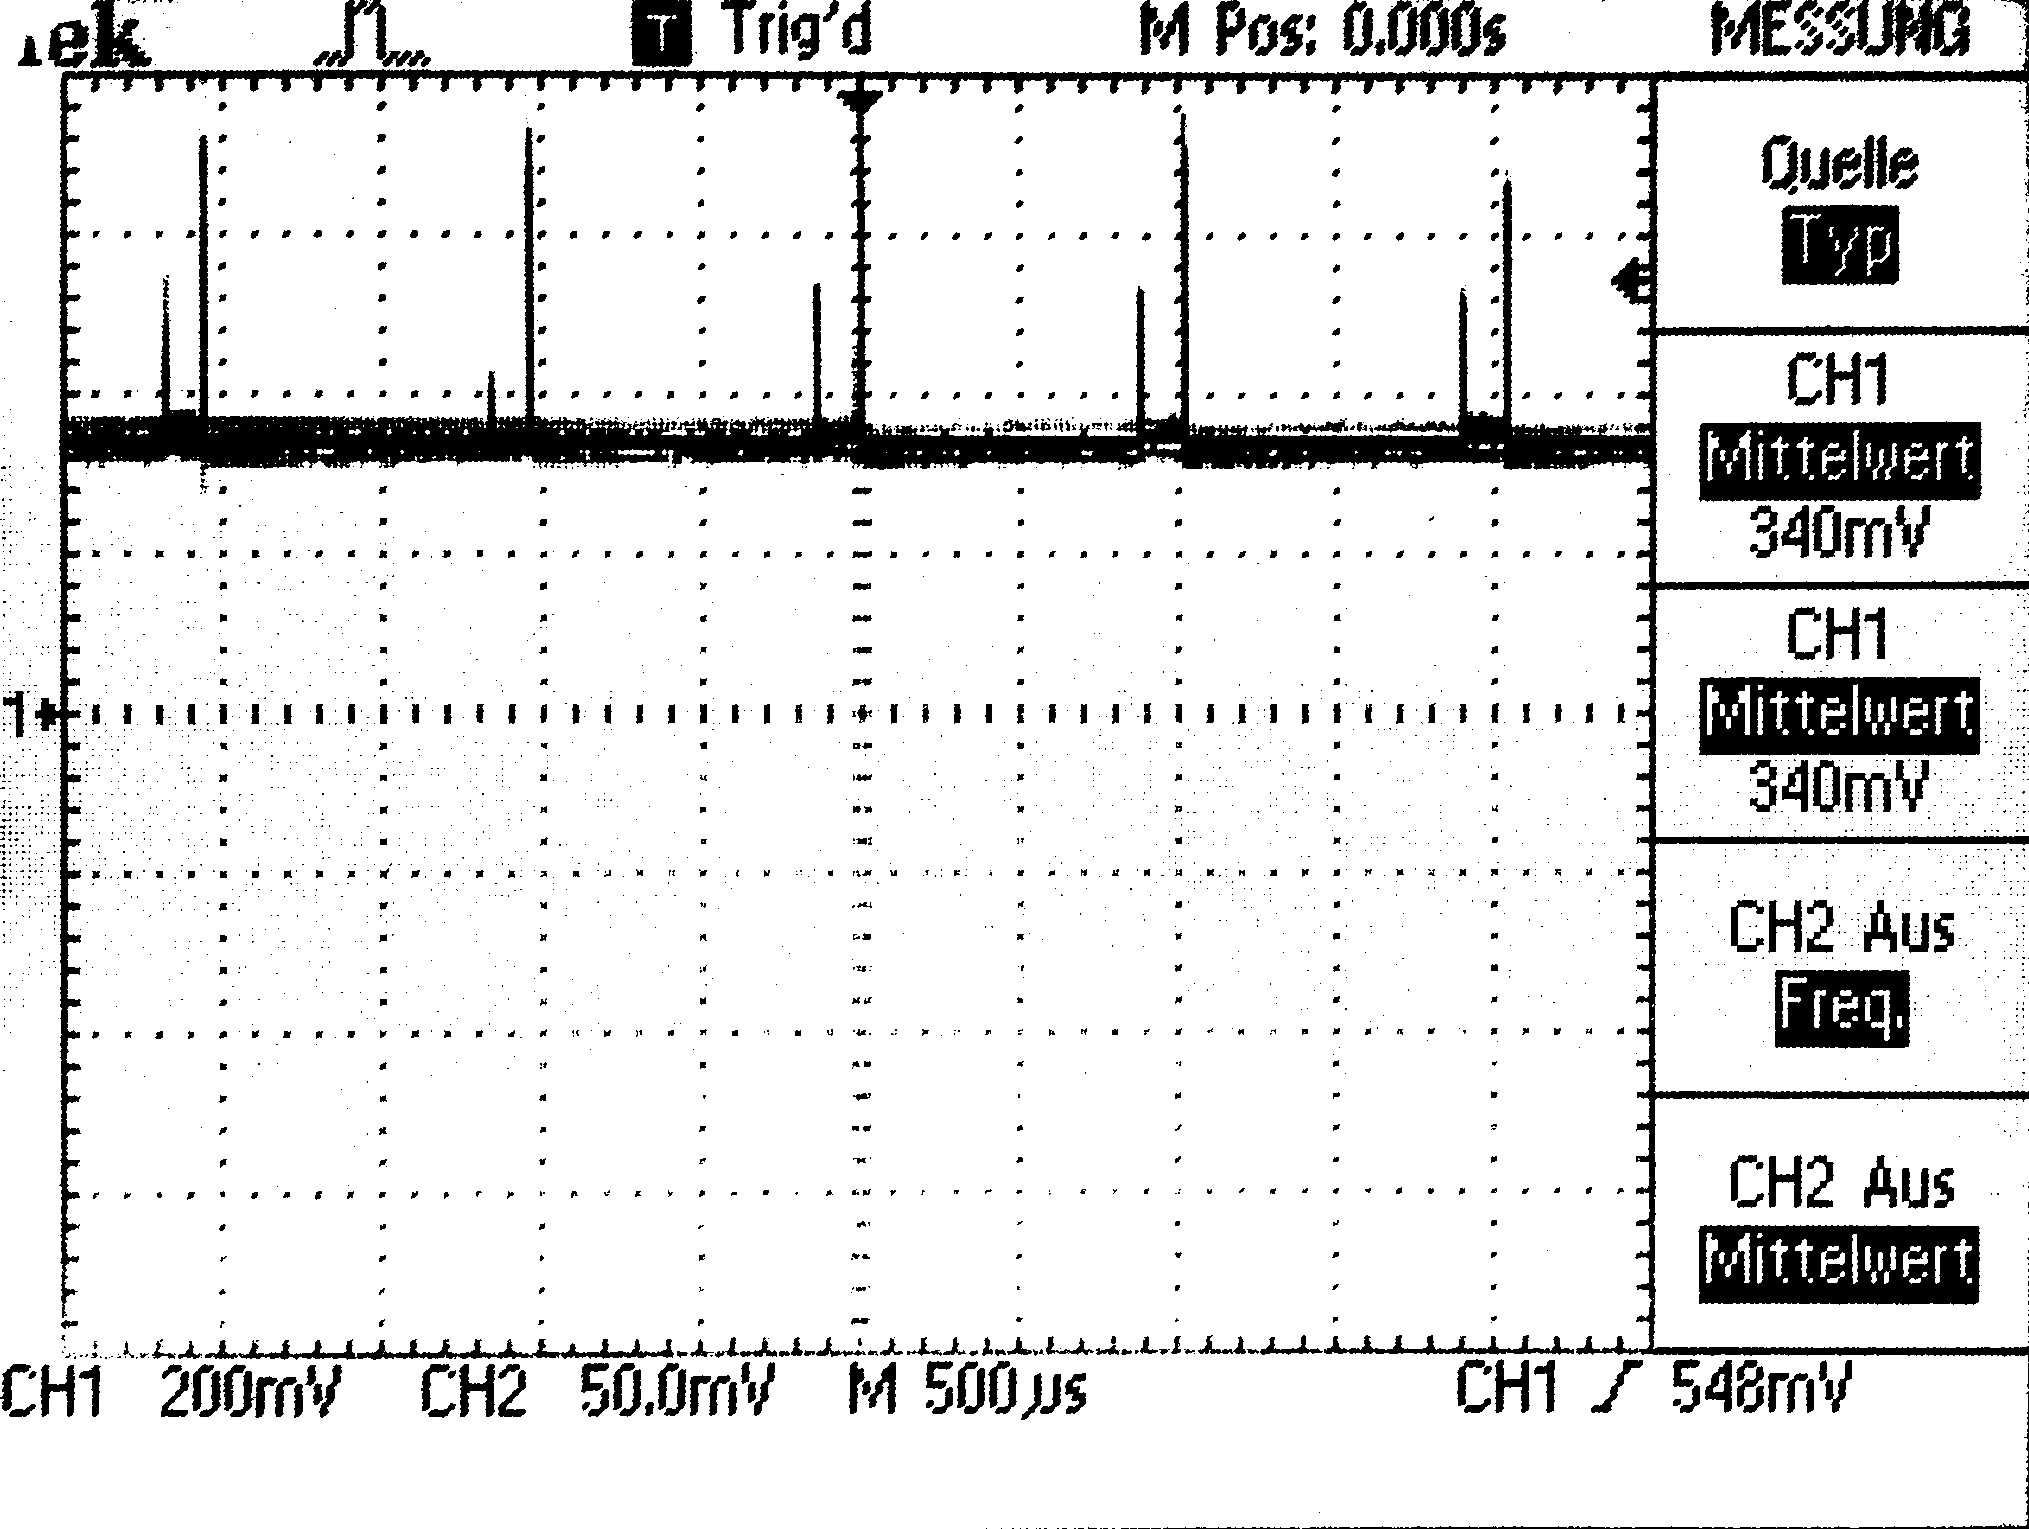
\includegraphics[width=.8\textwidth]{IR_spikes.png}\\
\caption{Ausgangssignal GP2D120}%
\label{fig:IR_spikes}
\end{figure}

Nach der Entstörung mit einem \SI{82}{\nano\farad} Kondensator direkt am Sensor zwischen VCC und GND sind die Störungen bereits stark vermindert.

\begin{figure}[H]
\centering
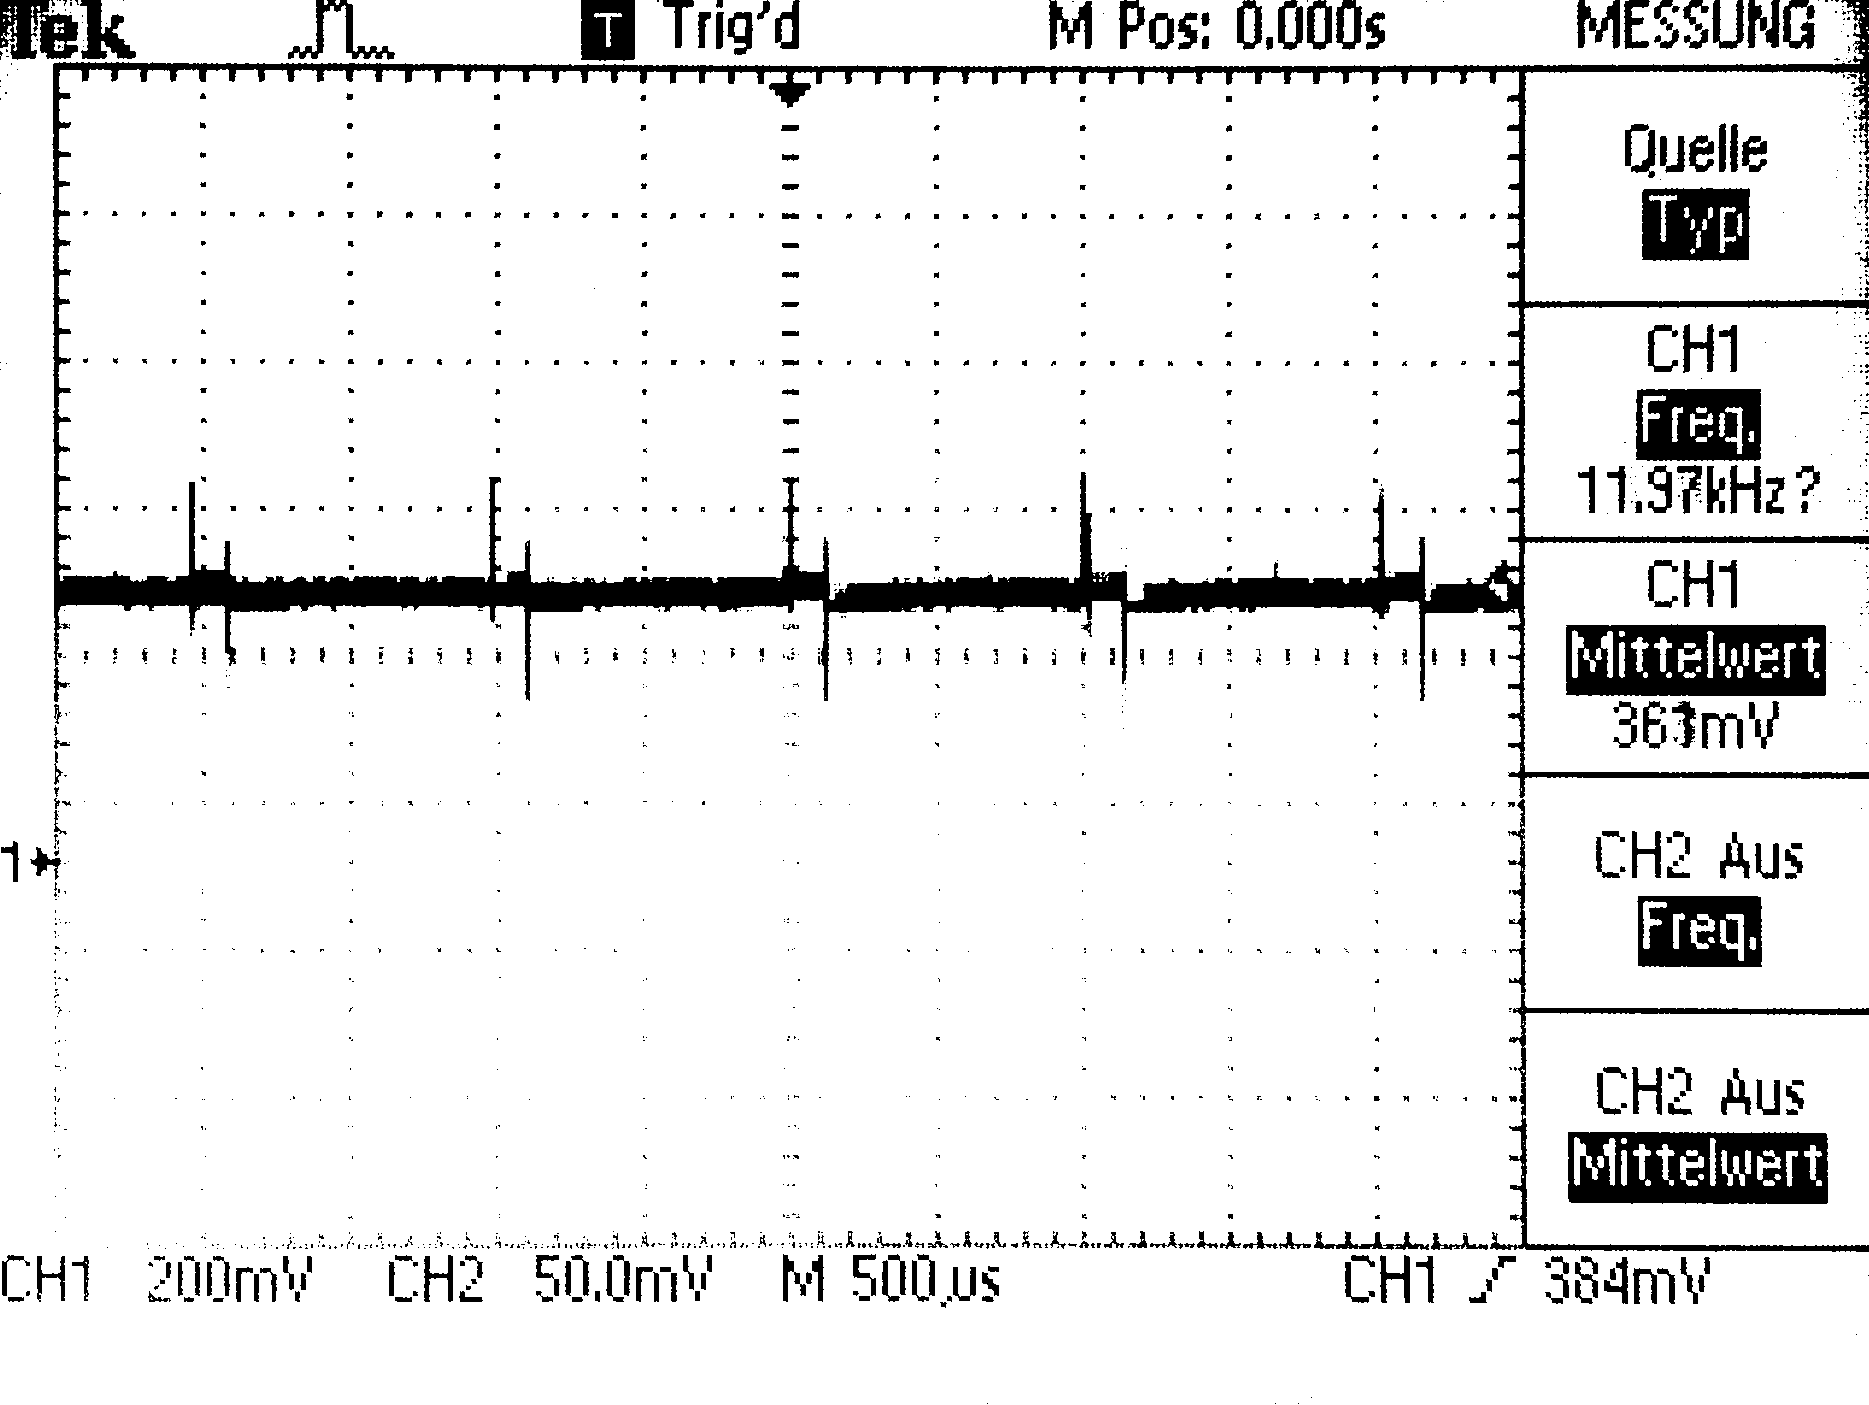
\includegraphics[width=.8\textwidth]{IR_lessspikes.png}\\
\caption{Ausgangssignal GP2D120 entstört}%
\label{fig:IR_lessspikes}
\end{figure}

Zusätzlich zum Kondensator direkt am Sensor werden diese noch mit einem \SI{47}{\micro\farad} Kondensator auf der Platine entkoppelt.

\subsection{Auswertung des Messsignales}
Das Messsignal vom Sensor wird über einen ADC-Eingang des AVR Mikrocontrollers ausgelesen. Angeschlossen werden die Sensoren über die PH-Connector Reihe des Herstellers JST, welche auch an den Sensoren verbaut sind.



\section{Odometrie}
Das Auto benötigt in unterschiedlichen Situationen unterschiedlich viel Leistung, um seine Geschwindigkeit zu halten.
Besonders in Kurven ist durch die erhöhte Reibung mehr Motorleistung nötig. Über den Motortreiber lässt sich jedoch nur
die mittlere Spannung am Motor verändern, deshalb ist es nötig diese zu regeln. Dafür ist jedoch eine Rückführung der Geschwindigkeit
des Autos nötig. Eine Aufintegrierung der Beschleunigungsdaten der Inertialsensorik führt auf Dauer zu erheblichen
Abweichungen und ist daher für eine Regelung nicht geeignet. Auch eine Odometrie an den Rädern des Autos ist
aus mechanischen Gründen schwer zu realisieren. 

Durch die feste Übersetzung des Getriebes bietet sich die Messung der Motordrehzahl an. Damit lässt sich eine gute Näherung für die aktuelle Geschwindigkeit erreichen. 

\subsection{Hall-Sensor}
Eine Möglichkeit die Motordrehzahl zu messen ist es das Magnetfeld des
Motorankers auszuwerten. Dazu sehen wir uns den Aufbau eines Gleichstrommotors an.
\begin{figure}[H]
\centering
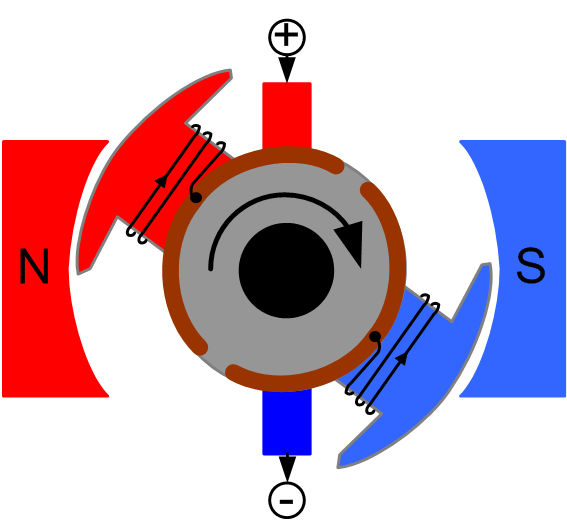
\includegraphics[width=.5\textwidth]{motor.png}\\
\caption{Aufbau eines Gleichstrommotors \cite{gs-motor}}%
\label{fig:aufbau_motor}
\end{figure}
Ein Gleichstrommotor besteht aus zwei grundsätzlichen Teilen, einem unbeweglichen Teil, den Stator und einem beweglichen Teil, dem Anker.
Der Stator besteht aus sich gegenüberliegenden Permanentmagneten, welche zwei entgegengesetzt gepolte Magnetfelder erzeugen.
Der Anker besteht aus Elektromagneten dessen Polung jede halbe Umdrehung kommutiert wird. Durch die Kommutierung ändert sich die 
Polung der Elektromagneten. Das sich so ändernde Magnetfeld kann mit einem Hallsensor ausgewertet werden. Das entstehende 
Signal ähnelt dabei über der Zeit einer Sinusschwingung. Mit Hilfe eines Schmitt-Trigger kann daraus ein Drehzahlsignal generiert werden.

Der Hallsensor ist erfolgreich durch ein Belüftungsloch im Motor platziert wurden. Als Referenzspannung für den Schmitt-Trigger wird der
Mittelwert des Sensorsignals, erzeugt durch einen Tiefpass, genutzt.

\begin{figure}[H]
\centering
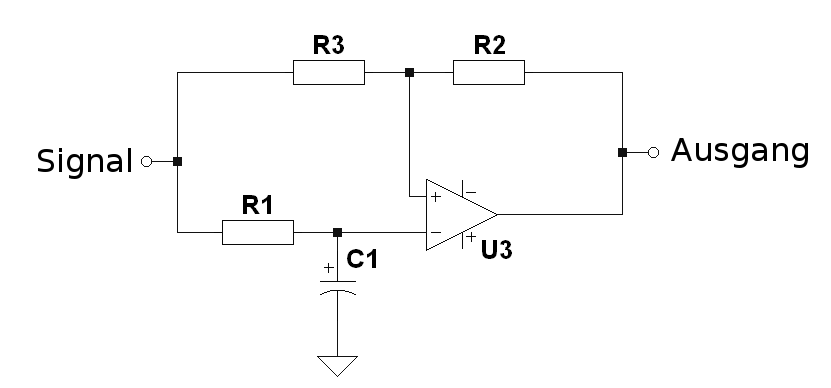
\includegraphics[width=.5\textwidth]{schmitt.png}\\
\caption{Schmitt-Trigger Schaltung}%
\label{fig:schmitt}
\end{figure}

Leider führt dieses Vorgehen nicht zum Erfolg, da die Magnetfeldstärke stark von der Drehrichtung des Motors abhängt. Es war nicht möglich
den Schmitt-Trigger so auszulegen, dass er in beide Drehrichtungen zuverlässig funktioniert.\\

Im Schaltplan befindet sich eine andere Schaltung, diese wurde aus Zeitnot kurz vor der Bestellung der Platine eingearbeitet und funktioniert ebenfalls nicht!

\subsection{Gabellichtschranke}

Alternativ zum Vorgehen mit einem Hall-Sensor wurde eine andere Lö\-sung implementiert. An eine speziell für diesen Motor angefertigte Achsverlängerung wurde eine Inkrementalgeberscheibe befestigt, zu sehen in \cref{fig:gabellichtschranke}. 
Diese wird durch einen Sharp GP1A30R Sensor ausgewertet, welcher ein Drehzahlsignal an den externen Takteingang des Timer 1 vom AVR Mikrocontroller liefert.
\begin{figure}[H]
\centering
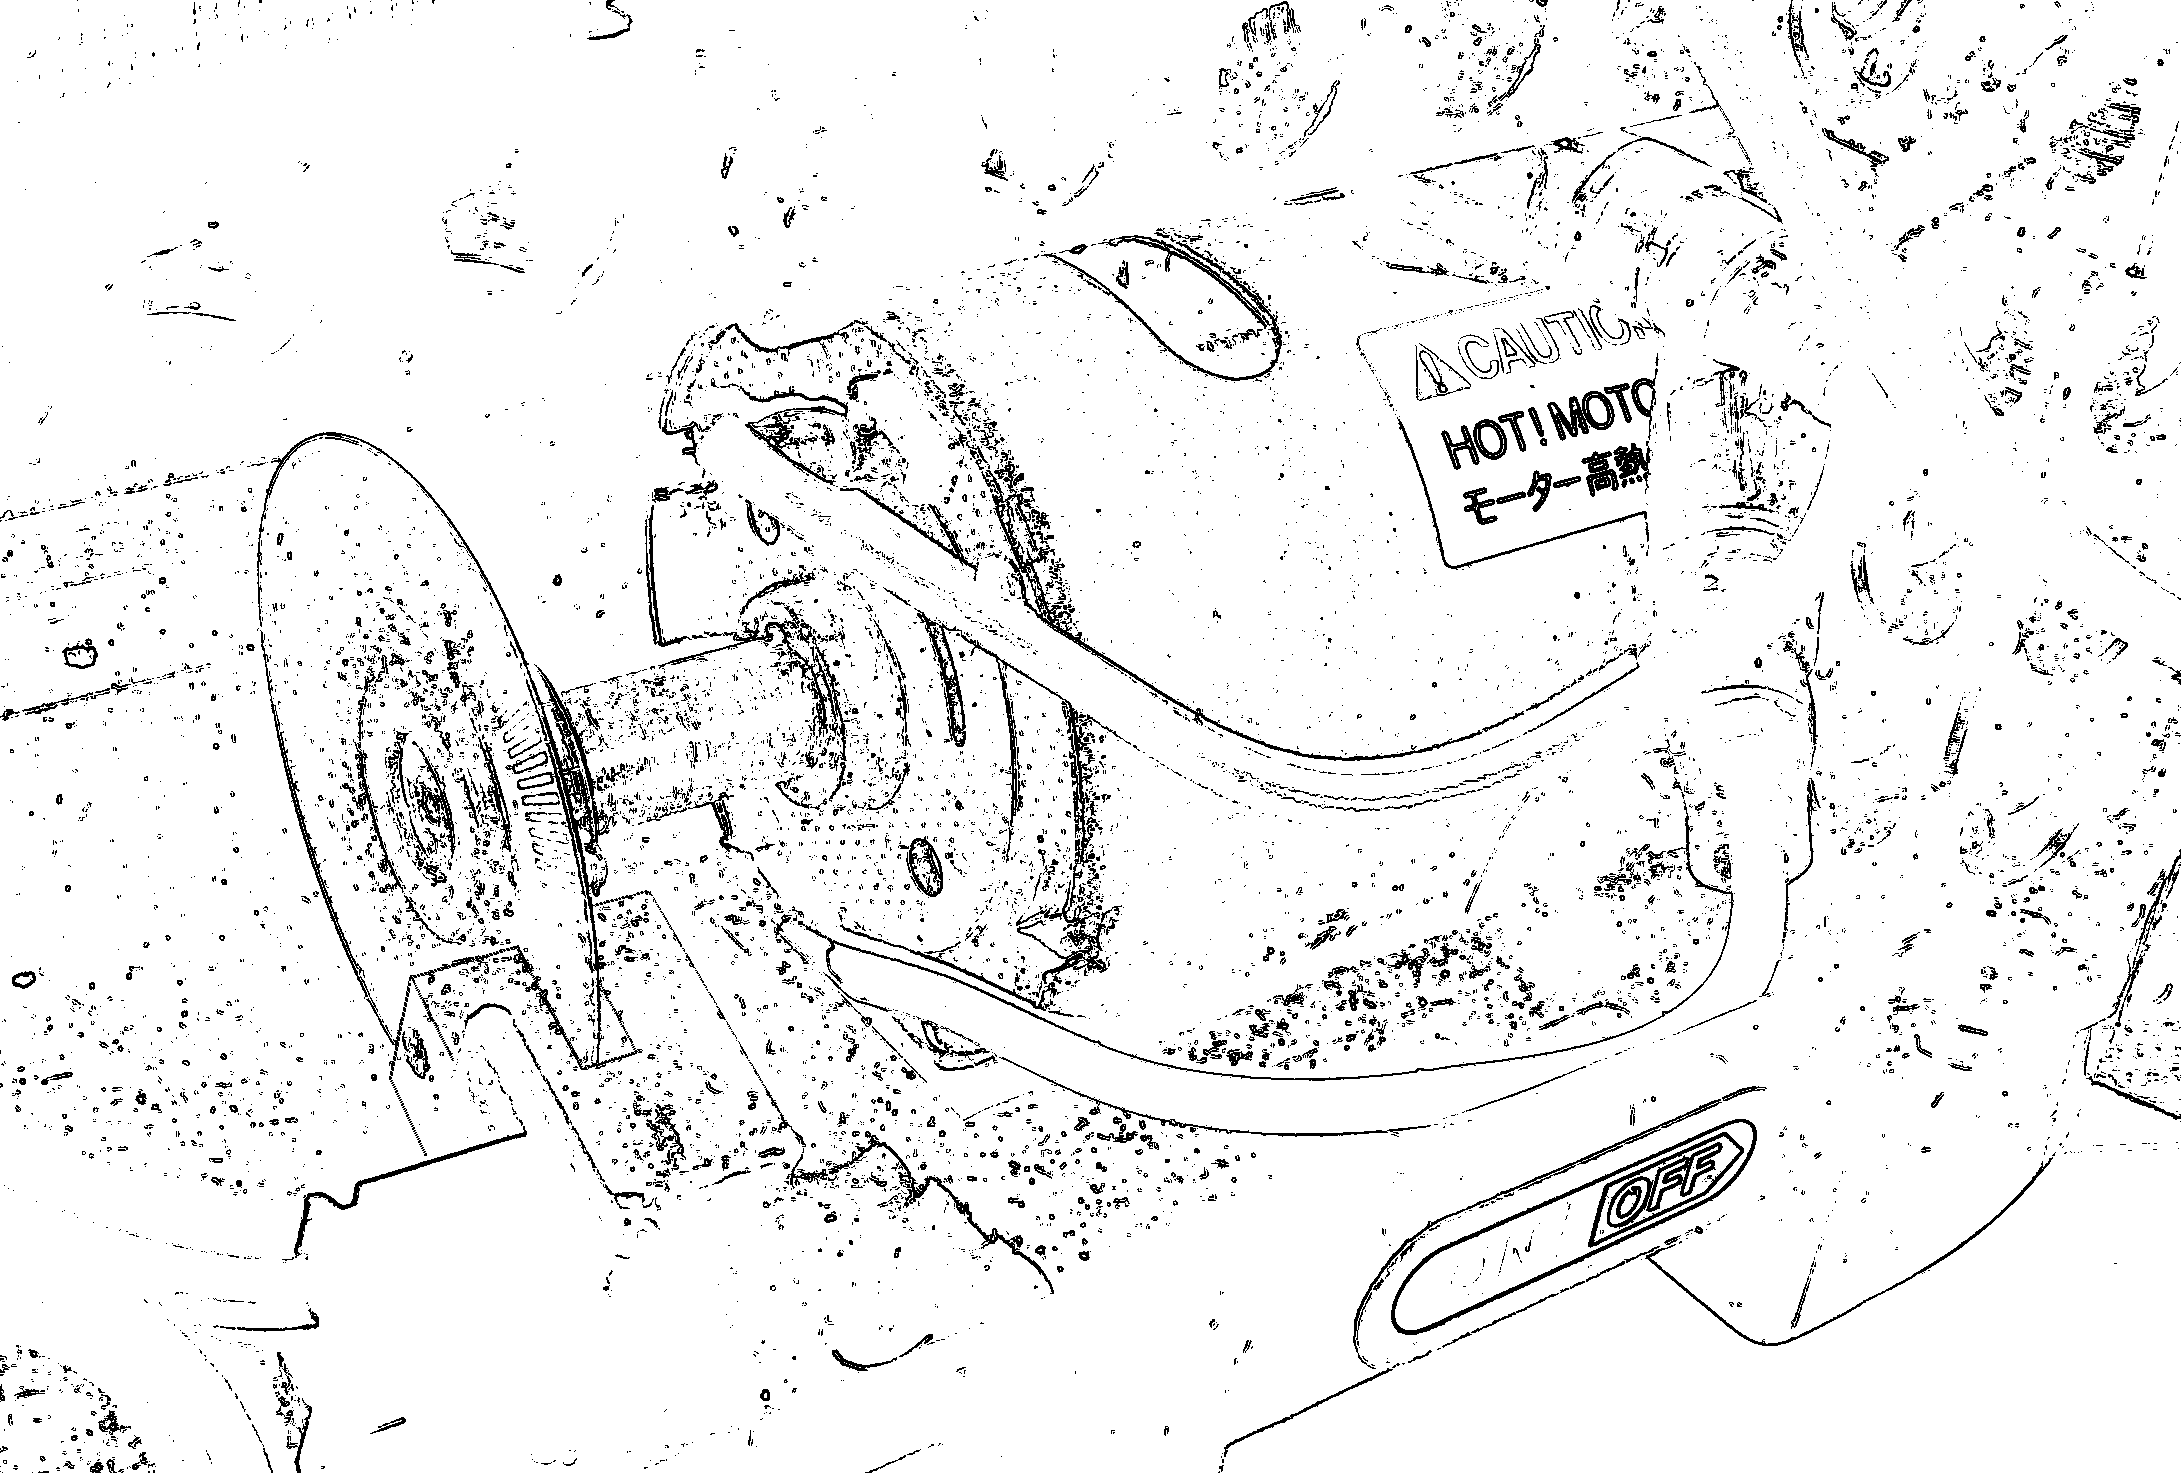
\includegraphics[width=.8\textwidth]{odometrie.png}\\
\caption{Motor mit Inkrementalgeber}%
\label{fig:gabellichtschranke}
\end{figure}

Die Scheibe ist dabei mit 120 Strichmarkierungen versehen. Eine Motorumdrehung entspricht also 120 Impulsen, im folgenden Motorticks genannt. Über das Übersetzungsverhältnis des Getriebes und dem Radumfang kann dann 
der zurückgelegte Weg berechnet werden. Das Übersetzungsverhältnis des Fahrzeugs ist abhängig von drei Komponenten, dem Stirnrad, dem Motorritzel sowie einer festen internen Übersetzung. Das verwendete Stirnrad hat
61 Zähne, das Motorritzel 19. Damit ergibt sich ein Verhältnis von 61:19 zusammen mit der internen Übersetzung von \num{2,6} \cite{uebersetzung}
haben wir ein Übersetzungsverhältnis von \num{8,35}. Der Radumfang beträgt ca. \SI{21}{\centi\meter}.

\begin{align}
\frac{120*8,35}{\SI{0,21}{\meter}}=\frac{ticks}{\si{\meter}}=4760
\end{align}

Mit dieser Größe lassen sich die Motorticks einfach in Meter umrechnen. 

\section{Auslegung der Stromversorgung}

Um das Layout der Platine möglichst simpel zu halten und damit kostengünstig zu bleiben, wurden alle Komponenten so ausgewählt, dass diese über eine einzige \SI{5}{\volt} Spannungsquelle mit Energie versorgt werden können.
Es ist wichtig den Stromverbrauch aller Komponenten abzuschätzen, um die Spannungsversorgung sinnvoll dimensionieren zu kön\-nen. Eine zu schwache Spannungsquelle kann zu Instabilitäten führen,
während eine überdimensionierte Geld verschenkt.

\subsection{Stromverbrauch der Komponenten}
In diesem Abschnitt soll eine Abschätzung des Stromverbrauchs vorgenommen werden. Dabei wird keinen Wert auf hohe Genauigkeit gelegt, es soll nur eine ungefähre Größenordnung für den Stromverbrauch gefunden werden.

\subsubsection{Servomotor}
Der Stromverbrauch des Servomotors ist schwer zu ermitteln. Da es sich um einen Modellbauservomotor handelt 
sind im Datenblatt hierzu keine Daten aufzufinden. Da ein Messaufbau für die Abschätzung des Stromverbrauches
zu aufwändig ist, werden hier Messwerte eines ähnlichen Servos aus einem Artikel \cite{website-servo} herangezogen.
Laut diesem hat eine Servomotor keinen konstanten Stromverbrauch. Der Stromfluss wird immer wieder unterbrochen, so dass es zu einem intervallartigen Stromfluss kommt.
Nur wenn der Servomotor dauerhaft belastet wird, kommt es zu einem konstanten Stromfluss.
Im Artikel werden mehrere Servomotoren vermessen, der Motor der dem verwendeten am nächsten kommt ist der ``Graupner 4421'' mit folgenden Daten:

%TODO
\todo{Servo Modell \cite{website-servo-dat} in Anforderungen mit aufnehmen}

Technische Daten ``Graupner 4421'' \cite{website-servo-vergleich-dat}:
\begin{itemize}
 \item Stellzeit(\SI{60}{\degree}): \SI{0,11}{\second}
 \item Stellmoment: \SI{88}{\newton\centi\meter} 
\end{itemize}


Technische Daten des verwendeten Servomotors \cite{website-servo-dat}:
\begin{itemize}
 \item Stellzeit(\SI{60}{\degree}): \SI{0,13}{\second} (\SI{4,8}{\volt}) / \SI{0,16}{\second} (\SI{6,0}{\volt})
 \item Stellmoment: \SI{92}{\newton\centi\meter} (\SI{4,8}{\volt}) / \SI{78}{\newton\centi\meter} (\SI{6,0}{\volt})
\end{itemize}



Dieser hat laut des Artikels eine maximale Stromaufnahme von \SI{1,2}{\ampere}. Um noch Luft nach oben zu haben wird hier ein Verbrauch von 
\SI{1,8}{\ampere} angenommen.

\subsubsection{Pandaboard ES}
Leider gibt es vom Hersteller des Pandaboards keine konkreten Angaben zum Stromverbrauch. Der Hersteller empfiehlt jedoch ein
Netzteil mit \SI{4}{\ampere}\cite{website-panda-supply}, wobei auch ein Betrieb an USB mit Hilfe eines Y-Kabels möglich ist. Die USB-2.0 Spezifikation\cite{website-usb-spec} sieht eine maximale 
Stromabgabe von \SI{500}{\milli\ampere} vor.

Der Stromverbrauch des normalen Pandaboards (ohne ES) beträgt ca. \SI{800}{\milli\ampere} \cite{website-panda-power}.
Nähere Angaben zum Stromverbrauch des normalen Pandaboards (ohne ES) finden sich in \cite{website-panda-power}.
Der Verbrauch des Pandaboard ES dürfte durch den schnelleren Prozessor minimal darüber liegen. 
Durch Anschluss von USB-Geräten an das Board kann der Stromverbrauch jedoch noch steigen. Die USB-Spezifikation \cite{website-usb-spec}
sieht pro Port eine maximale Stromentnahme von \SI{500}{\milli\ampere} vor. Da das Pandaboard über 2 USB-Ports verfügt, liegt der maximale zusätzliche Verbrauch bei \SI{1}{\ampere},
so dass hier ein Gesamtverbrauch von \SI{2}{\ampere} veranschlagt wird.

\paragraph{Hinweis:}
Das Pandaboard ES wurde im Laufe des Projekts durch einen Intel NUC ersetzt, welcher jedoch nicht über die \SI{5}{\volt} Schiene versorgt wird.
Daher entfällt der Verbrauch des Boards in den Messungen der Evaluierung.

\subsubsection{LED Beleuchtung}
Auch wenn LEDs den Ruf haben besonders energieeffizient zu sein, ist der Stromverbrauch bei einer größeren Anzahl nicht zu
unterschätzen. Da wir RBG-LEDs einsetzen besteht ein LED-Modul aus 3 LEDs in den Grundfarben rot, blau und grün.
Laut Datenblatt \cite{ds-WS2812} haben die LEDs eine Stromaufnahme von \SI{20}{\milli\ampere}, also \SI{60}{\milli\ampere} pro Modul.
Um regelwerkkonform zu sein, werden folgende Beleuchtungen benötigt: Blinker rechts und links jeweils vorne und hinten.
Sowie eine Leuchte, welche den RC-Modus anzeigt. Zusätzlich zu den im Regelwerk vorgeschriebenen Beleuchtungen werden noch je
zwei Frontscheinwerfer und drei Rück-/Bremslichter integriert, so dass sich eine Anzahl von 10 LED-Modulen ergibt.
Der maximale durch die LEDs verursachte Strom liegt somit bei \SI{600}{\milli\ampere}. 

\subsubsection{Mikrocontroller}
Der maximale Stromverbrauch des AVR Mikrocontrollers liegt laut Datenblatt\cite{ds-at90can} bei \SI{200}{\milli\ampere}, wenn IO-Pins belastet werden
Der Mikrocontroller selber braucht jedoch bei \SI{5}{\volt} Betriebsspannung und 16MHz nur \SI{29}{\milli\ampere}. Da die IO-Pins des Controllers nur wenig belastet werden,
wird hier nur ein Verbrauch von \SI{100}{\milli\ampere} veranschlagt.

\subsubsection{Sharp Sensoren}
Die Sharp GP2D120 Distanzsensoren verbrauchen laut Datenblatt \cite{ds-sharp-GP2D120} \SI{50}{\milli\ampere}, da zwei dieser Sensoren verbaut werden ergeben sich \SI{100}{\milli\ampere}.

\subsubsection{Sonstige Peripherie}
Da der Stromverbrauch der restlichen Komponenten minimal ist, werden hier pauschal \SI{100}{\milli\ampere} veranschlagt.

\subsection{Auswahl des Reglers}
Der Gesamtstromverbrauch der Komponenten beträgt \SI{4800}{\milli\ampere}. Ein Linearregler ist hier nicht mehr praktikabel, da dieser bei einer Akkuspannung von \SI{14,4}{\volt} und \SI{4800}{\milli\ampere} über \SI{45}{\watt} Leistung in Wärme umwandeln würde.

\begin{align*}
P_{\text{linear}}=(\SI{14,4}{\volt}-\SI{5}{\volt})\cdot \SI{4,8}{\ampere}=\SI{45,120}{\watt}
\end{align*}

Schaltregler in Form von Abwärtswandlern haben hingegen einen sehr hohen Wirkungsgrad. Eine gute Wahl ist die Schaltregler-Reihe von Texas Instuments, da diese einfach zu bekommen sind,
und nur wenig Außenbeschaltung benötigen. Ein Exemplar das unseren Anforderungen entspricht ist der LM2678 von Texas Instruments, dieser kann dauerhaft einen Strom von \SI{5}{\volt} liefern und sein Wirkungsgrad
liegt selbst bei Maximallast bei über 80\%.
Eine Übersicht dazu findet sich in \cref{fig:vreg-eff}.
\begin{figure}[H]
\centering
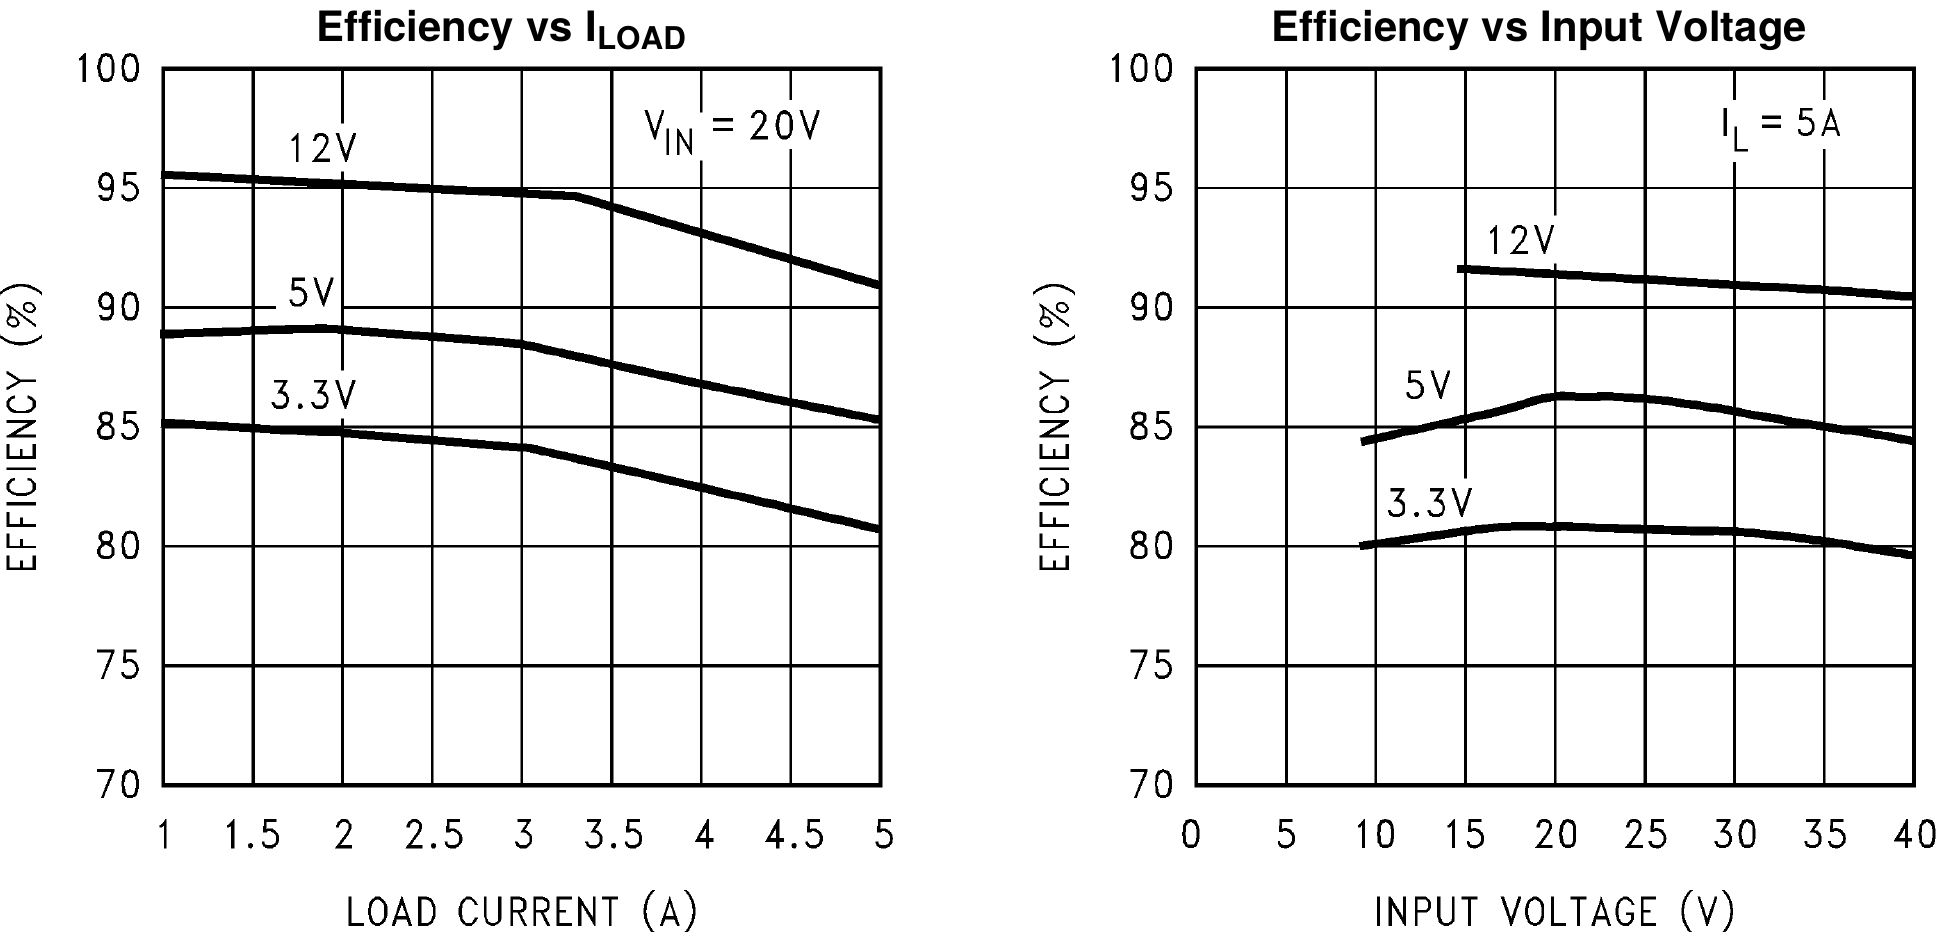
\includegraphics[width=.8\textwidth]{vreg.png}\\
\caption{Regulator Wirkungsgrad \cite{ds-ti}}%
\label{fig:vreg-eff}
\end{figure}
Ausgehend von ca. \SI{24}{\watt} Leistungsaufnahme ($\SI{4,8}{\ampere}*\SI{5}{\volt}$) und einem minimalen Wirkungsgrad von 80\%  ergibt sich damit eine überschauliche Verlustleistung von \SI{6}{\watt}.


\begin{figure}[H]
\centering
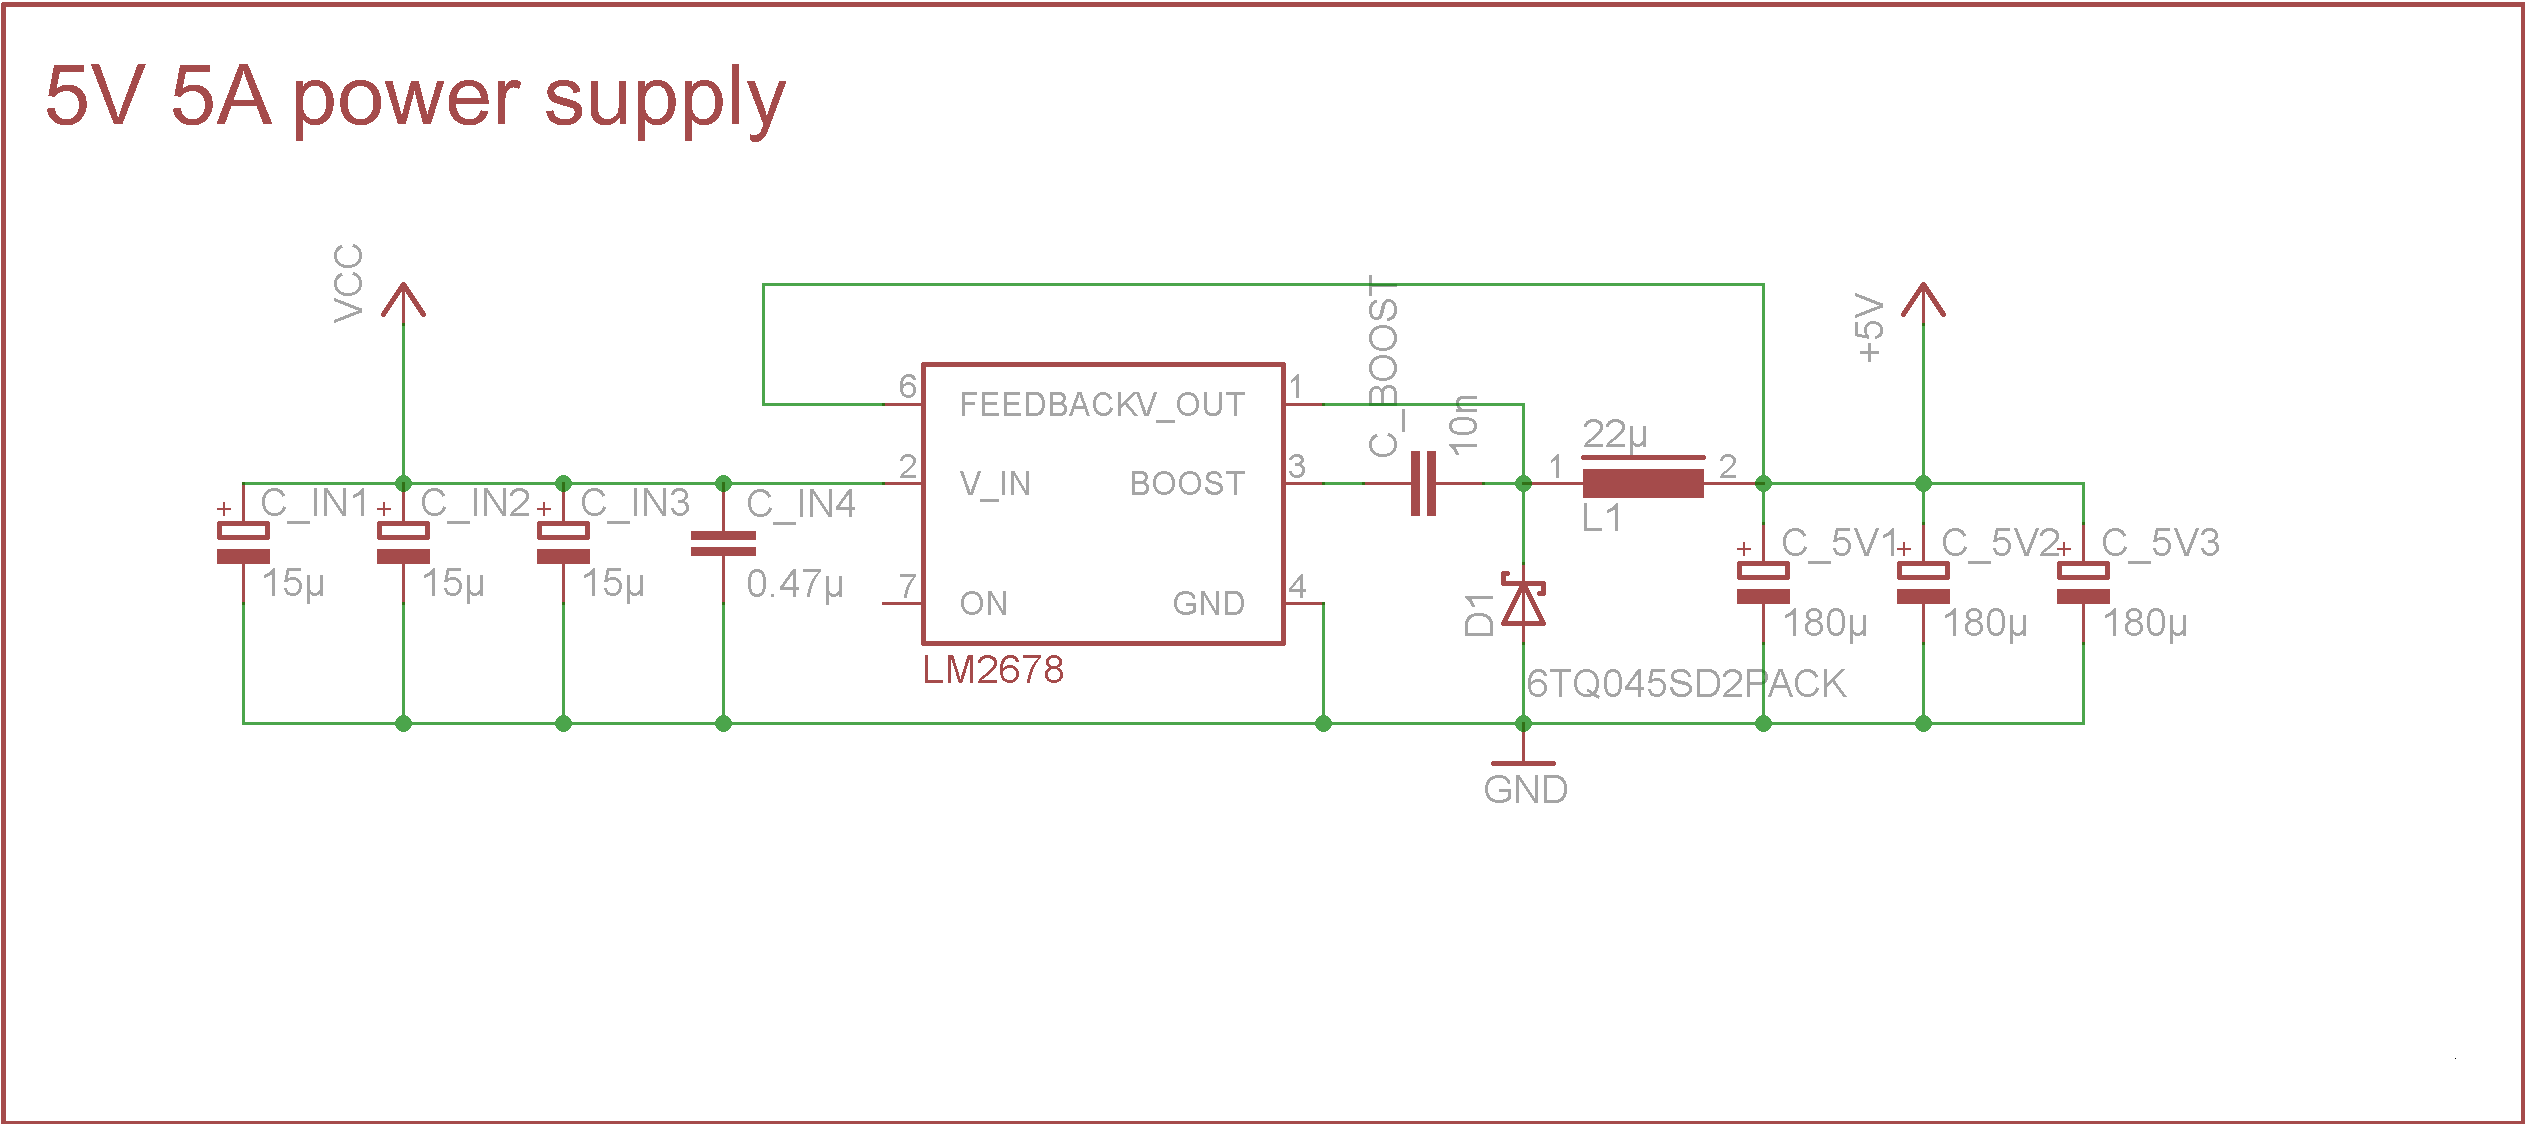
\includegraphics[width=\textwidth]{5vregler.png}\\
\caption{Schaltplan des 5V Reglers}%
\label{fig:vreg}
\end{figure}


Die Beschaltung erfolgt dabei nach den Empfehlungen des Datenblattes. Die verwendeten \SI{180}{\micro\farad} Kondensatoren sollen laut Datenblatt Low-ESR Kondensatoren sein. 
Die verbauten Kondensatoren stammen aus Nichicons L8 Serie und haben einen Serienwiderstand von nur \SI{12}{\milli\ohm}.

\textbf{Low-ESR Kondensatoren:\\}

Low-ESR Kondensatoren zeichnen sich durch einen niedrigen Serienwiderstand ($R_{ESR}$) aus.
Dieser liegt in Reihe(Serie) zum idealen Kondensator (\cref{fig:esr}). 

\begin{figure}[H]
\centering
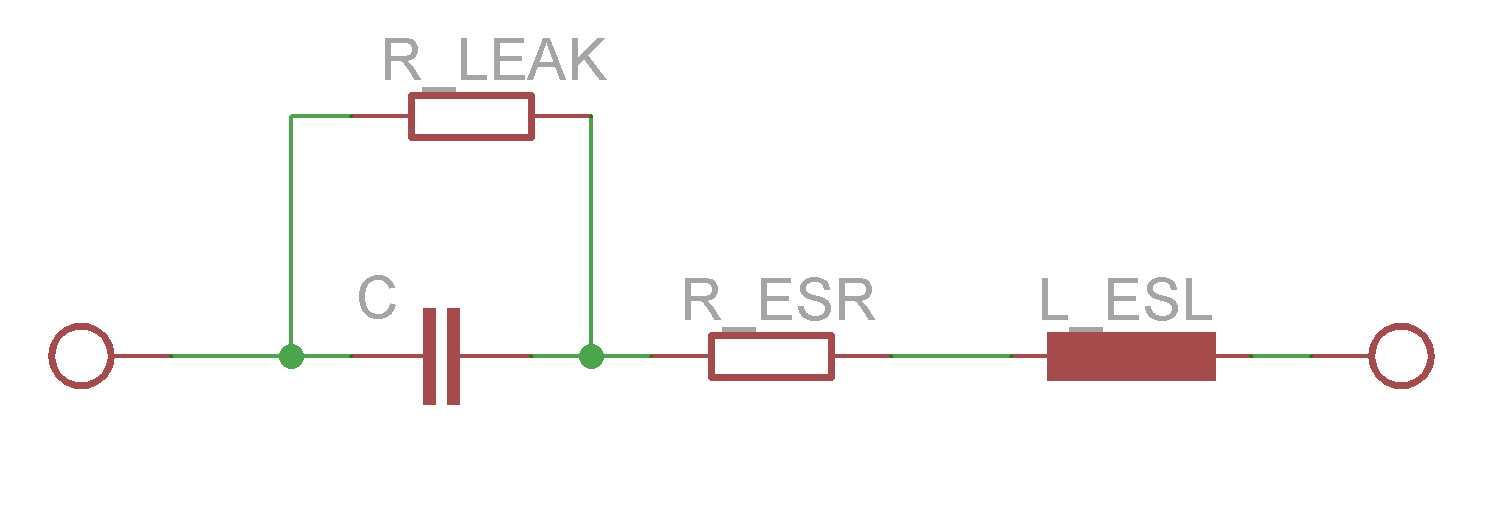
\includegraphics[width=.56\textwidth]{esr.png}\\
\caption{Ersatzschaltbild eines Kondensators}%
\label{fig:esr}
\end{figure}

Dieser verursacht Verluste innerhalb des Kondensators, was bei Belastung zur Erwärmung des Kondensators führt und
seine Lebensdauer verringert. Je kleiner der ESR desto niedriger die Verluste im Kondensator. Weiterhin
kann ein Kondensator mit kleinem ESR schneller ge- und entladen werden, als ein herkömmlicher Kondensator.
%Im entlade Fall kann man sich den Kondensator als Spannungsquelle vorstellen, der ESR stellt dann den Innenwiderstand der Spannungsquelle dar.
Durch diese Eigenschaften ist ein ESR Kondensator hervorragend zur Störunterdrückung geeignet.






\section{Das Layout}
In \cref{fig:layout} ist das fertige Platinenlayout zu sehen. Bei der Entwicklung des Layouts wurde darauf geachtet, dass die Platine in die vorgesehene Lücke (zu sehen in \cref{fig:car_struc}) des Fahrzeugs passt.

\begin{figure}[H]
\centering
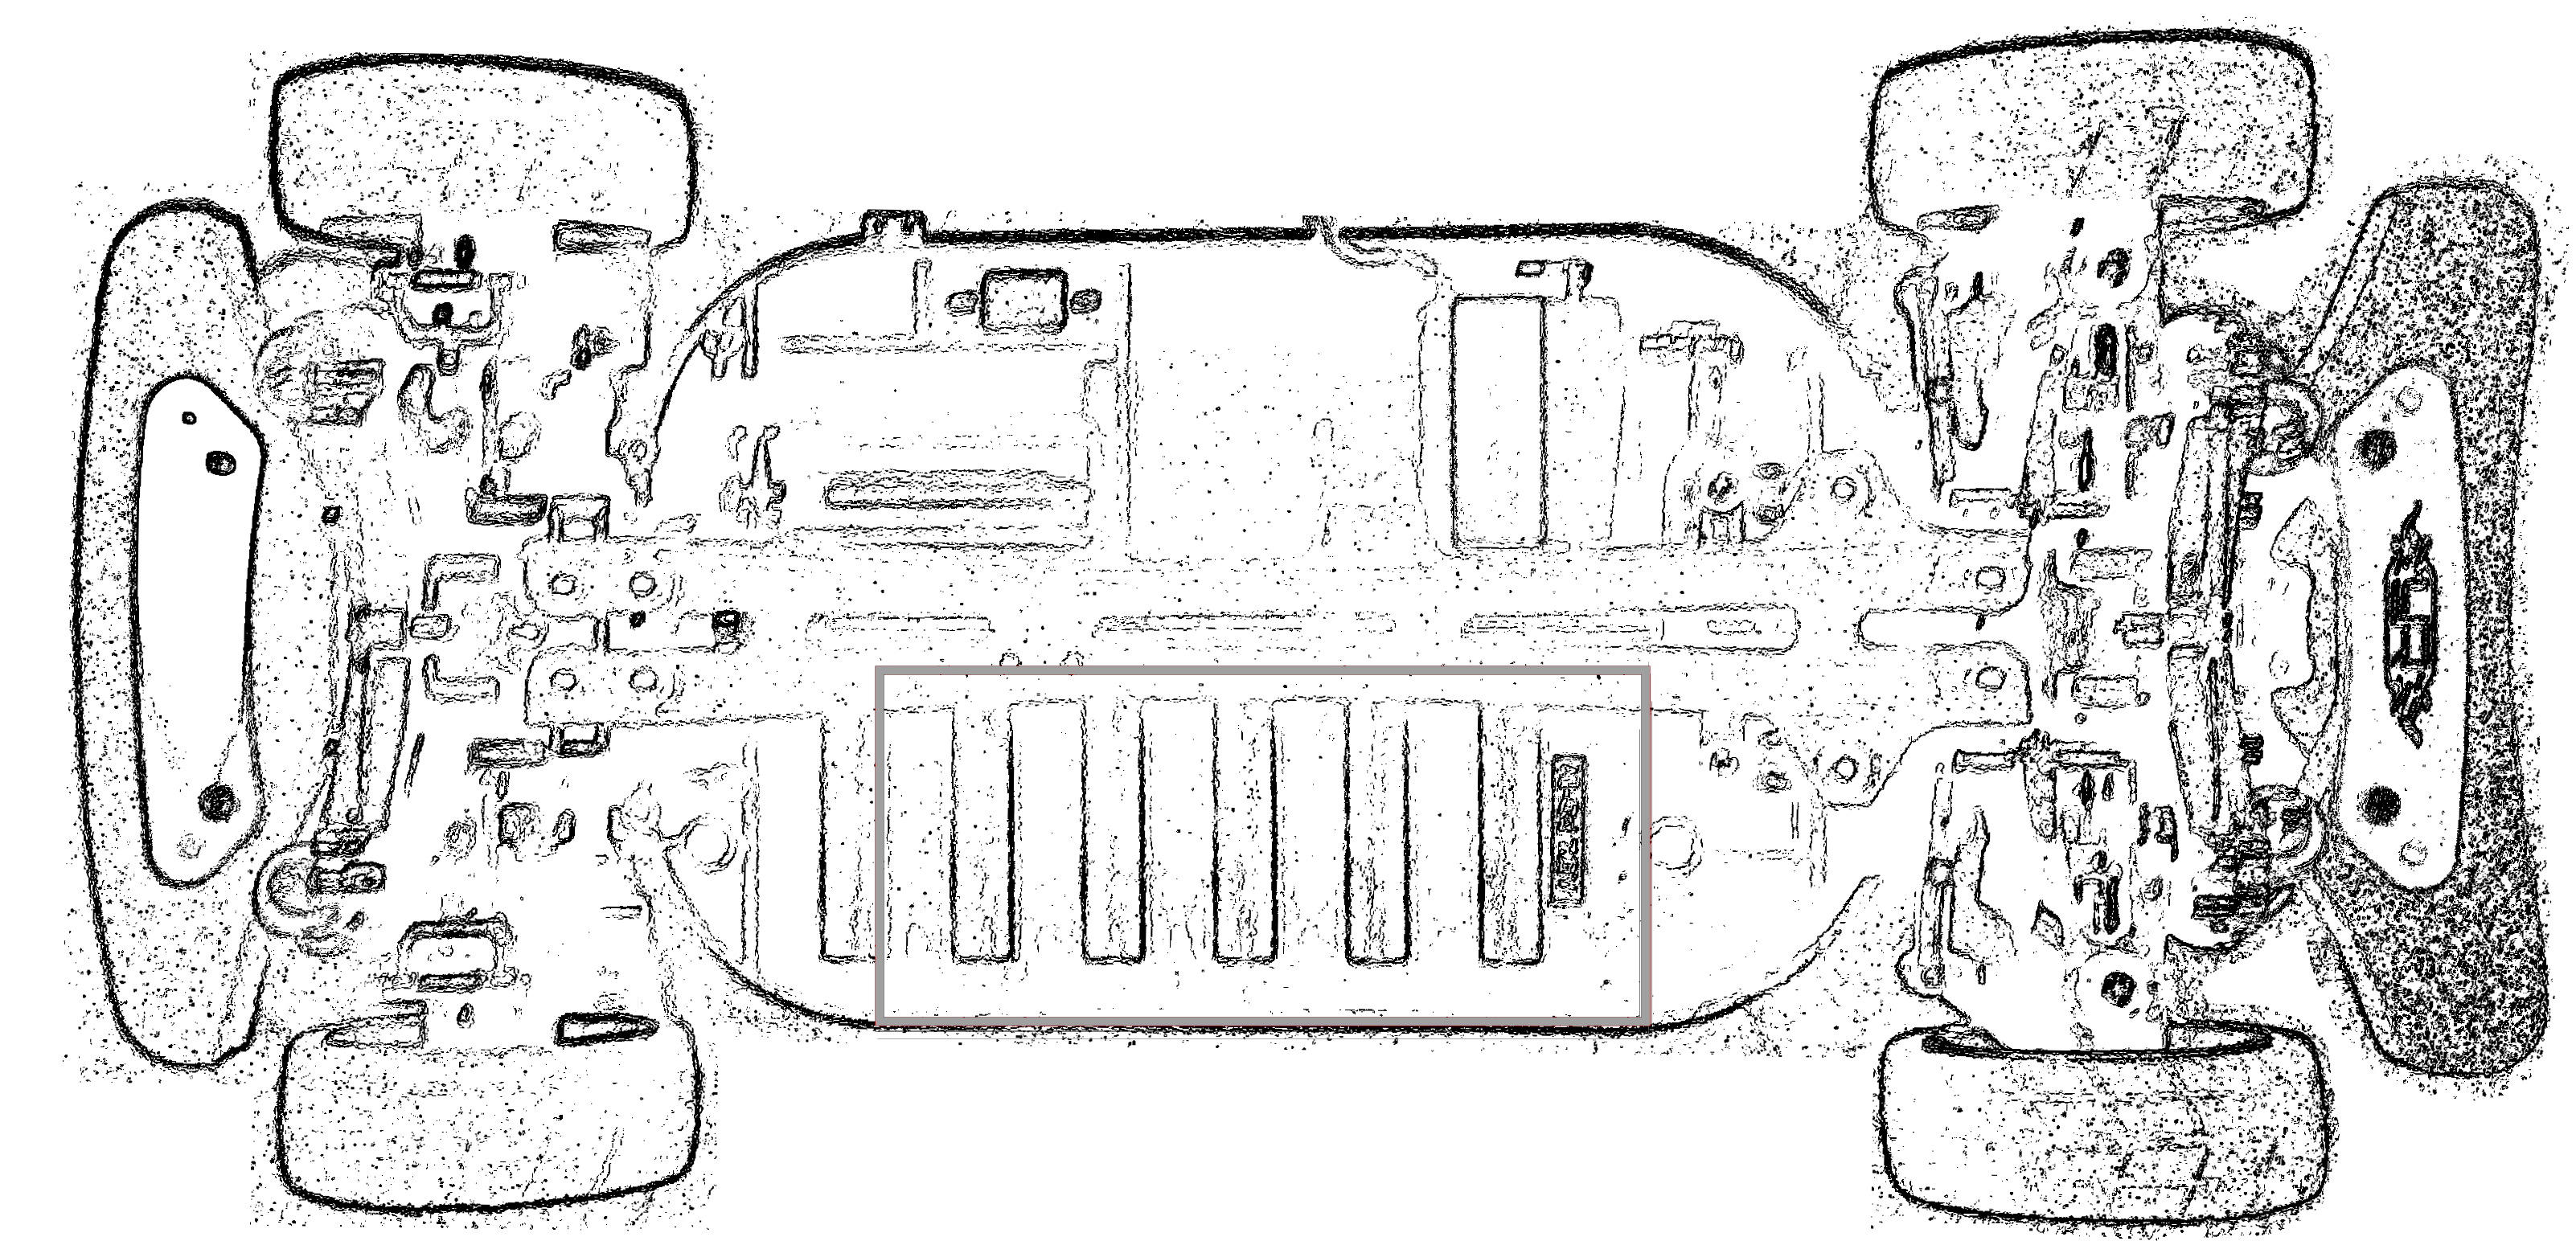
\includegraphics[width=.8\textwidth]{auto_struck.png}\\
\caption{Fahrzeug Platinen-Position}%
\label{fig:car_struc}
\end{figure}

Die Lücke hat Maße von \SI{13,0}{\centi\meter} mal \SI{5,4}{\centi\meter}. Das Platinenlayout hat eine Größe von  \SI{13,0}{\centi\meter} mal \SI{5,05}{\centi\meter} und passt somit in die Lücke ohne dabei zu viel Spielraum zu haben, 
was in einem festen Sitz der Platine resultiert. 

\begin{figure}[H]
\centering
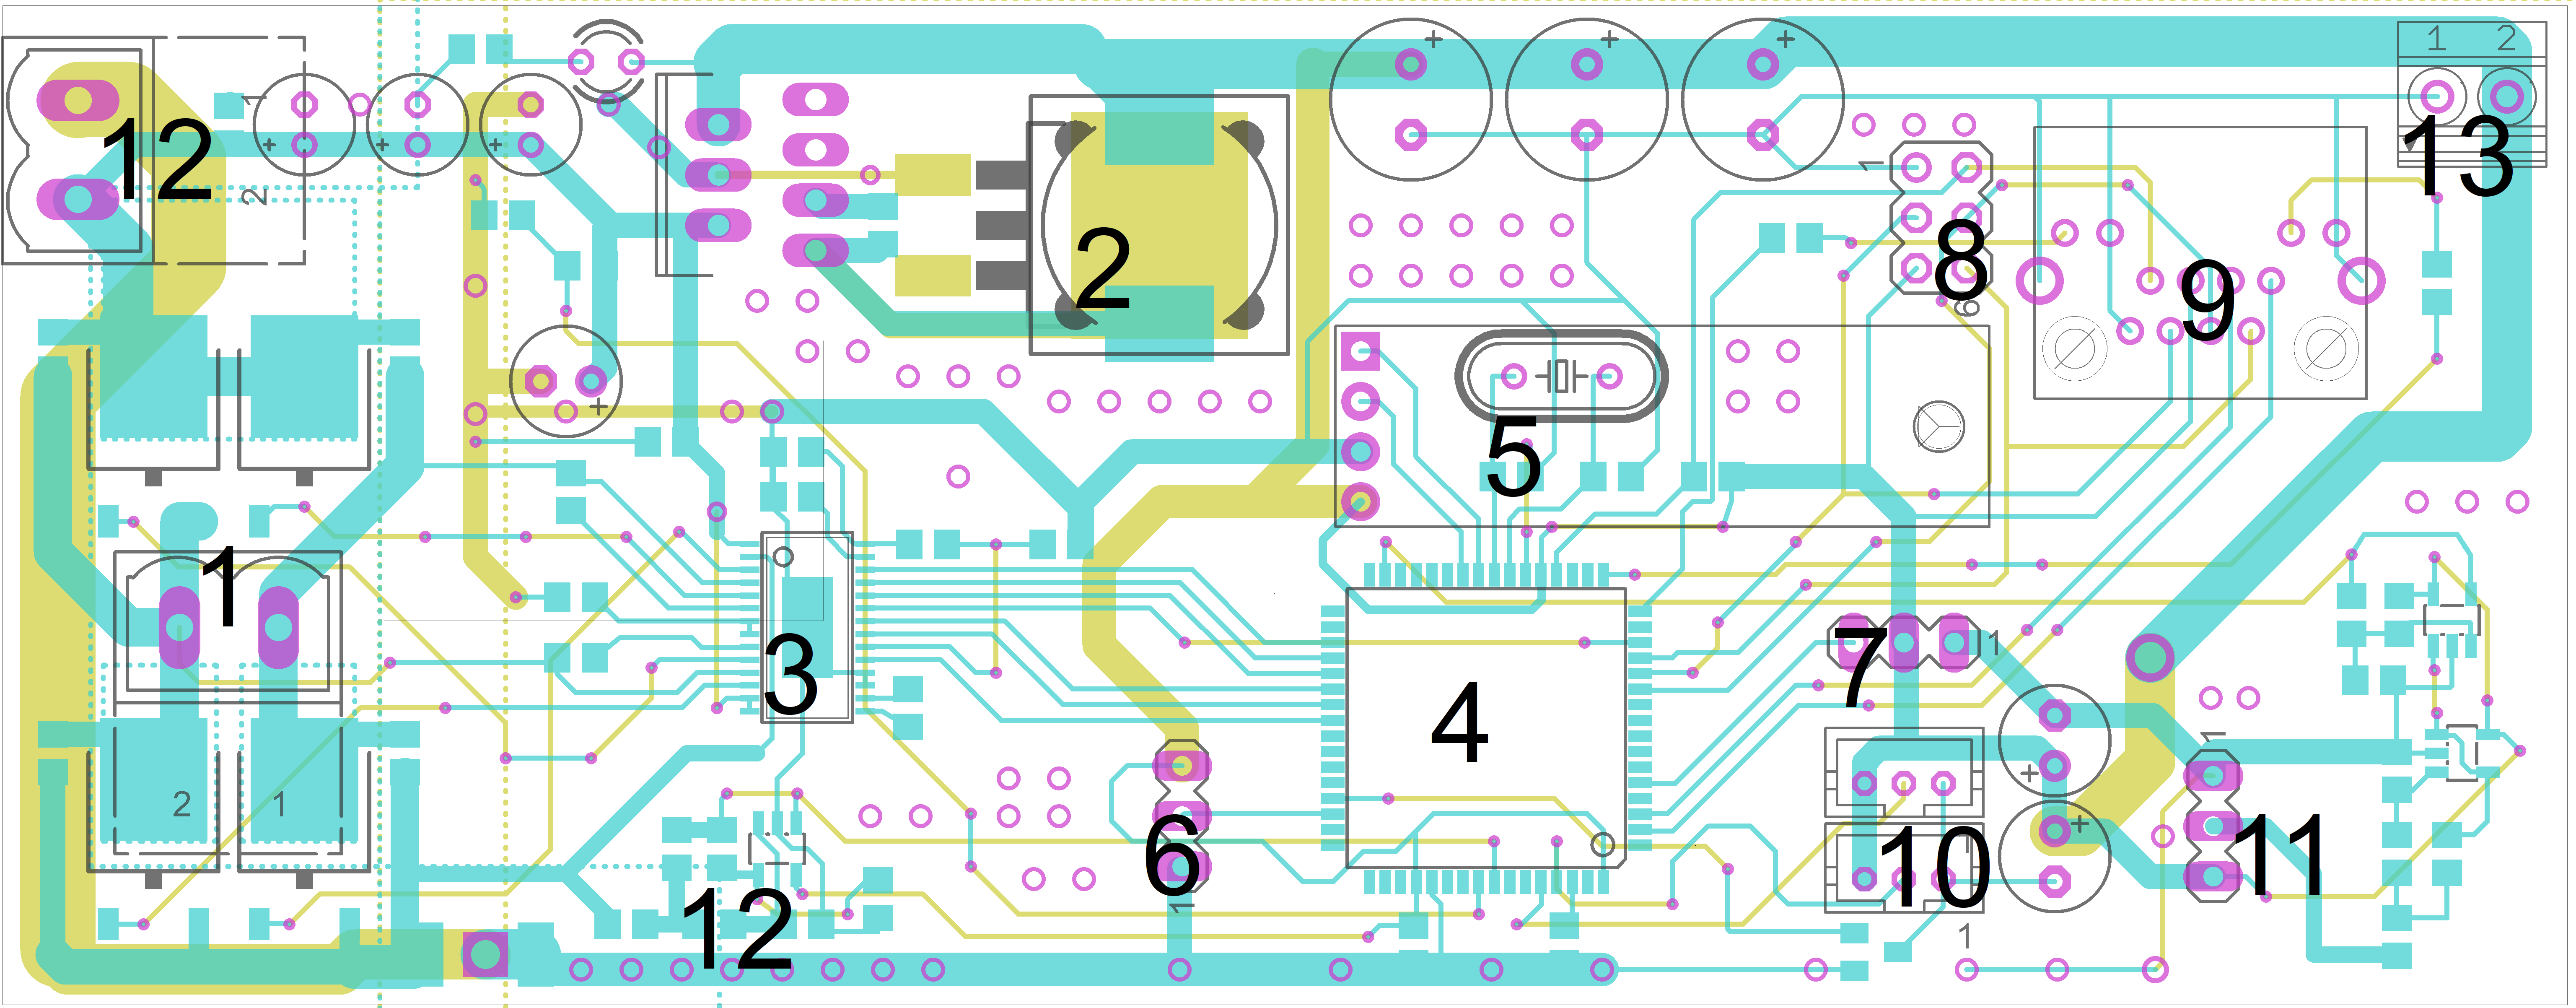
\includegraphics[width=.8\textwidth]{platinen_layout_scr.png}\\
\caption{Platinenlayout}%
\label{fig:layout}
\end{figure}


Auf dem Layout sind folgende Komponenten zu sehen:
\begin{itemize}
\setlength{\parskip}{0pt}
 \item [1] H-Brücke mit Motoranschluss
 \item [2] \SI{5}{\ampere} Schaltregler
 \item [3] Allegro Mosfettreiber
 \item [4] Atmel Mikrocontroller
 \item [5] Sparkfun Inertialsensor (Anschluss und Position)
 \item [6] Anschluss für den LED-Strang
 \item [7] Anschluss für den Servomotor
 \item [8] ISP Anschluss zum Programmieren des Mikrocontrollers
 \item [9] RJ45 Buchse zum Anschluss der Pandaboards (mit SPI und U\-ART)
 \item [10] Anschlüsse für die Sharp GP2D Sensoren 
 \item [11] Anschluss und Filterschaltung für die Odometrie (Hallsensor)
 \item [12] Shunt mit Filterschaltung zur Strommessung
 \item [13] Stromanschluss für die Pandaboards
\end{itemize}



\section{Software}

Die Software besteht im Grunde aus zwei Teilen, zum einem der Firmware auf dem Mikrocontroller zum anderem aus der Software auf der Recheneinheit, welche die Daten vom Mikrocontroller ausliest und über ROS published.
In den folgenden Abschnitten werden erst die beiden Softwareteile erläutert und dann wird das Übertragungsprotokoll ver\-an\-schau\-licht.


\subsection{Software auf dem Mikrocontroller}
Die Software auf dem Mikrocontroller ist vollständig in C++ geschrieben. Eine vollständige Dokumentation der Software ist als Doxygen Dokument verfügbar. 
Die Software fungiert auf dem Controller als Service und wartet legendlich auf eine Anfrage von der seriellen Schnittstelle, welche sie bearbeitet und bei Bedarf beantwortet. 


\subsection{Client Programm auf der Recheneinheit}
Das Client Programm, im folgenden SerialNode genannt, wurde zuerst in Python implementiert. Durch die Verwendung der pyserial Bibliothek zum Ansprechen der seriellen Schnittstelle wurde jedoch
eine enorm hohe CPU-Last verursacht. Da sich das Problem kurzfristig nicht lösen ließ, die Rechenleistung für andere Aufgaben benötigt wird und auch Energieeffizienz ein wichtiges Kriterium ist,
wurde das Programm erneut in C++ implementiert. Unter Verwendung der Systemaufrufe von Poll konnte das Abfragen der seriellen Schnittstelle auf Systemebene ausgeführt werden, was die Effizienz stark 
verbesserte. Während die Python Implementierung einen CPU-Kern zu 100\% auslastete liegt die C++ Implementierung im unteren einstelligen Prozentbereich.
Eine vollständige Dokumentation der Software ist ebenfalls als Doxygen Dokument verfügbar.

Das Programm stellt nach seinem Start folgende ROS-Topics zur Ver\-fü\-gung:\\
 
\begin{table}[H]
  \centering
  \begin{tabularx}{\textwidth}{|l|l|}
    \hline
     Ros-Topic 			& Ros-Datentyp			 \\ \hline \hline	
    /sensors/current		& std\_msgs/Float32														\\ \hline
    \multicolumn{2}{|X|}{Der aktuelle Motorstrom in Ampere}											\\ \hline\hline
    /sensors/imu/data\_raw	& ottocar\_msgs/simpleImu													\\ \hline
    \multicolumn{2}{|X|}{Die Daten werden im ROS-Standardformat für Inertialsensoren zur Verfügung gestellt	}						\\ \hline\hline
    /sensors/IR1		& std\_msgs/Float32										\\ \hline
     \multicolumn{2}{|X|}{Der aktuelle Spannungswert des Sensors in Volt}										\\ \hline\hline
    /sensors/IR2		& std\_msgs/Float32										\\ \hline
      \multicolumn{2}{|X|}{Der aktuelle Spannungswert des Sensors in Volt}										\\ \hline\hline
    /sensors/motor\_revolutions	& std\_msgs/UInt32										\\ \hline
      \multicolumn{2}{|X|}{Die Anzahl der vergangenden Motorumdrehungen seit dem Start des Mikrocontrollers}						\\ \hline\hline
    /sensors/motor\_state	& std\_msgs/UInt8										\\ \hline
      \multicolumn{2}{|X|}{Der aktuelle Zustand des Motortreibers}											\\ \hline\hline
    /uC\_time			& std\_msgs/UInt32										\\ \hline
      \multicolumn{2}{|X|}{Die vergangene Zeit auf dem Mikrocontrollers seit dessen Start in Millisekunden}						\\ \hline\hline
    /sensors/voltage		& std\_msgs/Float32										\\ \hline
     \multicolumn{2}{|X|}{Die aktuelle Akkuspannung in Volt}												\\ \hline

  \end{tabularx}
  \caption{ROS-Publisher}%
  \label{tab:ros-pub}
\end{table}


Das Programm hört auf folgende ROS-Topics:\\

\begin{table}[H]
  \centering
  \begin{tabularx}{\textwidth}{|l|l|}
    \hline
     Ros-Topic 			& Ros-Datentyp			 	\\ \hline\hline
    /actuators/speed\_cmd		& std\_msgs/Int8										\\ \hline	
      \multicolumn{2}{|X|}{Die neue Motorgeschwindigkeit von -128 bis +127}		\\ \hline\hline
    /actuators/angle\_cmd		& std\_msgs/Int8										\\ \hline	
     \multicolumn{2}{|X|}{Der neue Servowinkel von -128 bis +127}			\\ \hline\hline
    /actuators/motor\_reset		& std\_msgs/Bool										\\ \hline	
     \multicolumn{2}{|X|}{Initiiere einen Reset im Motortreiber}			\\ \hline
  \end{tabularx}
  \caption{Ros-Subscriber}%
  \label{tab:ros-sub}
\end{table}



\subsection{Übertragungsprotokoll}
Da die Übertragung der Daten via ROS-Serial im ersten Prototypen zu vielen Problemen geführt hat, wurde ein neues Übertragungsprotokoll entwickelt.
Dabei wurde auf Fehlertoleranz und niedrigen Ressourcenverbrauch geachtet. Der Datendurchsatz muss hier ausreichend sein, um alle Daten stabil mit \SI{100}{\hertz}
übertragen zu können.
Der grundlegende Ablauf der Datenübertragung ist in \cref{fig:uC_read} und \ref{fig:uC_write} zu sehen.

Während eines Lesevorganges (\cref{fig:uC_read}) wartet der Mikrocontroller auf ein fest definiertes Startsignal von der Recheneinheit. Nachdem das Startsignal empfangen wurde, wird auf eine weitere Preamble gewartet.
Dies ist notwendig, um bei Asynchronitäten die Wahrscheinlichkeit eines zufälligen Startsignals zu verringern. Wurde die Preamble erfolgreich empfangen, erwartet der Mikrocontroller eine gültige Topic ID.
Wurde eine falsche Preamble empfangen, wartet der Mikrocontroller erneut auf ein gültiges Startsignal. Abhängig von der Topic ID verfährt der Mikrocontroller dann im Programm fort und beantwortet
die Anfrage entsprechend. Für manche Topics ist eine Bestätigung (Acknowledge) nötig. Bekommt der Mikrocontroller keine Bestätigung sendet er die Daten erneut. Eine Bestätigung wird nur gesendet,
wenn die vom Client berechnete Checksumme mit der mitgesendeten identisch ist. Dies ist besonders bei den Daten der Inertialsensorik von Nöten, da hier defekte Daten zu einem dauerhaften Fehler führen. 
Die Anzahl dieser Retransmits ist begrenzt und wird vom Client festgelegt. Wurde ein Acknowledge empfangen oder für den Topic ist keine Bestätigung
nötig, wartet der Controller erneut auf ein Startsignal.

\begin{figure}[ht]
\centering
\includegraphics[page=1,width=.8\textwidth]{graph/read.pdf} 
\caption{Lese Daten}
\label{fig:uC_read}
\end{figure}

Der Ablauf eines Schreibvorganges (\cref{fig:uC_write}) auf dem Mikrocontroller ist ähnlich. Der Mikrocontroller wartet auf das Startsignal und eine Preamble sowie eine Topic ID.
Nach dem Empfang der Topic ID erwartet er die nötigen Daten, samt Checksumme. Diese ist nötig, um die Daten zu verifizieren. Bei der Ansteuerung des Motors kann ein
Bitfehler zu fatalen Folgen führen. Beispielsweise kann die Recheneinheit oder der Mikrocontroller abstürzen, wenn die Motorleistung plötzlich stark erhöht wird.
Daher werden die Daten nur übernommen, wenn die Checksumme erfolgreich verifiziert wurde. Sollte die Checksumme nicht verifiziert werden, springt der Mikrocontroller
erneut in den Startzustand und wartet auf ein Startsignal, ohne die Daten zu übernehmen. Der Client bekommt davon nichts mit, wenige einzelne Fehler können durch die
hohe interne Datenrate von \SI{100}{\hertz} ignoriert werden. Häufige oder dauerhafte Fehlübertragungen können durch die Reaktion des Autos leicht identifiziert werden.
Häufige oder dauerhafte Fehlübertragungen würden durch das fortlaufende Lesen und Schreiben auf dem Mikrocontroller so oder so zu Fehlern in beiden Richtungen führen.

\begin{figure}[ht]
\centering
\includegraphics[page=1,width=.8\textwidth]{graph/write.pdf} 
\caption{Schreibe Daten}
\label{fig:uC_write}
\end{figure}





